% SIAM Article Template
\documentclass[review,onefignum,onetabnum]{siamart171218}

% Information that is shared between the article and the supplement
% (title and author information, macros, packages, etc.) goes into
% ex_shared.tex. If there is no supplement, this file can be included
% directly.

% SIAM Shared Information Template
% This is information that is shared between the main document and any
% supplement. If no supplement is required, then this information can
% be included directly in the main document.


% Packages and macros go here
\usepackage{lipsum}
\usepackage{amsfonts}
\usepackage{graphicx}
\usepackage{epstopdf}
\usepackage{algorithmic}
\ifpdf
  \DeclareGraphicsExtensions{.eps,.pdf,.png,.jpg}
\else
  \DeclareGraphicsExtensions{.eps}
\fi

% Add a serial/Oxford comma by default.
\newcommand{\creflastconjunction}{, and~}

% Used for creating new theorem and remark environments
\newsiamremark{remark}{Remark}
\newsiamremark{hypothesis}{Hypothesis}
\crefname{hypothesis}{Hypothesis}{Hypotheses}
\newsiamthm{claim}{Claim}

% Sets running headers as well as PDF title and authors
\headers{Greedy parameter selection for one-way spatial marching}{M.K. Sleeman, and Tim Colonius}

% Title. If the supplement option is on, then "Supplementary Material"
% is automatically inserted before the title.
\title{Greedy recursion parameter selection for one-way spatial integration of hyperbolic equations\thanks{Submitted to the editors October 21, 2025.
\funding{This work was funded by The Boeing Company through the Strategic Research and Development Relationship
Agreement CT-BA-GTA-1.}}}

% Authors: full names plus addresses.
\author{Michael K.\ Sleeman\thanks{California Institute of Technology, Pasadena, CA 
  (\email{msleeman@caltech.edu}).}
\and Tim Colonius\footnotemark[1]}

\usepackage{amsopn}
\DeclareMathOperator{\diag}{diag}


%% Added on Overleaf: enabling xr
\makeatletter
\newcommand*{\addFileDependency}[1]{% argument=file name and extension
  \typeout{(#1)}% latexmk will find this if $recorder=0 (however, in that case, it will ignore #1 if it is a .aux or .pdf file etc and it exists! if it doesn't exist, it will appear in the list of dependents regardless)
  \@addtofilelist{#1}% if you want it to appear in \listfiles, not really necessary and latexmk doesn't use this
  \IfFileExists{#1}{}{\typeout{No file #1.}}% latexmk will find this message if #1 doesn't exist (yet)
}
\makeatother

\newcommand*{\myexternaldocument}[1]{%
    \externaldocument{#1}%
    \addFileDependency{#1.tex}%
    \addFileDependency{#1.aux}%
}
%%% END HELPER CODE
%%% Local Variables: 
%%% mode:latex
%%% TeX-master: "ex_article"
%%% End: 


% Optional PDF information
\ifpdf
\hypersetup{
  pdftitle={GreedyOWNS},
  pdfauthor={M.K. Sleeman, and T. Colonius}
}
\fi

% The next statement enables references to information in the
% supplement. See the xr-hyperref package for details.

%% Use \myexternaldocument on Overleaf
\myexternaldocument{ex_supplement}

% FundRef data to be entered by SIAM
%<funding-group>
%<award-group>
%<funding-source>
%<named-content content-type="funder-name"> 
%</named-content> 
%<named-content content-type="funder-identifier"> 
%</named-content>
%</funding-source>
%<award-id> </award-id>
%</award-group>
%</funding-group>

\usepackage{bm}
\usepackage{subcaption}

% comment
\usepackage{xcolor}
\newcommand{\michael}[1]{\textcolor{magenta}{Michael: #1}}

\begin{document}

\maketitle

% REQUIRED
\begin{abstract}
Solutions to hyperbolic systems comprise waves propagating at finite speeds. When wave propagation is predominantly unidirectional, one-way wave equations can be used to evolve only the right-going solution by removing support for left-going waves. The One-Way Navier-Stokes (OWNS) approach, which was originally developed for systems of first-order hyperbolic equations, constructs one-way approximations to the linearized Navier-Stokes equations using a recursive filter to remove left-going waves. The computational cost scales with the number of recursion parameters, which must be carefully chosen to ensure accuracy and stability of the resulting one-way equation. Previous work has chosen parameters based on heuristic estimates of key eigenvalues, which requires trial-and-error tuning while also yielding slow error convergence. We propose a greedy algorithm for automatic parameter selection, which we show yields faster convergence and a net decrease in computational cost for linear and nonlinear disturbance evolution in boundary-layer flows. We review the OWNS projection (OWNS-P) and recursive (OWNS-R) methods, comparing their convergence properties, and show through our numerical analysis and experiments that OWNS-P yields superior convergence and stability properties. Although we demonstrate the method for Navier-Stokes equations, we perform our analyses on systems of linear first-order hyperbolic equations, and emphasize that the greedy algorithm is applicable to such systems.
\end{abstract}

% REQUIRED
\begin{keywords}
  hyperbolic, one-way equation, parabolic approximation, greedy algorithm, spatial marching
\end{keywords}

% REQUIRED
\begin{AMS}
35L50, 65M99, 76E09
\end{AMS}

\section{Introduction}

Wave propagation can be modeled by (linear) systems of first-order hyperbolic partial differential equations (PDEs), solvable either as time-domain initial boundary value problems or frequency-domain boundary value problems. When wave propagation is predominantly unidirectional, one-way wave equations can be used to evolve the right-going solution by removing support for left-going waves. Such equations can be obtained by factoring the dispersion relation in Fourier–Laplace space into left- and right-going factors, and then retaining only the right-going branch. Since the resulting equation contains a square root of the Fourier-Laplace variables, the transformation back to physical space results in a nonlocal integro-differential equation, which can be localized using rational approximations of the square root~\cite{Lee_2000_Parabolic}. Although these methods are accurate, well-posed, and efficient for simple wave equations~\cite{Trefethen_1986_Parabolic,Halpern_1988_OneWay} such as the equations for geophysical migration of seismic waves~\cite{Claerbout_1976_Geophysics,Claerbout_1985_Geophysics} and underwater acoustics~\cite{Collins_1989_Underwater,Jensen_1995_Underwater}, they can only be applied in cases where the eigenvalues can be determined analytically, since the dispersion relation must be factored analytically. Methods for one-way marching that do not depend on this factorization have been developed by Guddati~\cite{Guddati_2006_OneWay} for acoustic and elastic wave equations, and by Towne and Colonius~\cite{Towne_2015_OWNS-O} for general systems of first-order hyperbolic equations.

While the linearized Euler equations comprise a system of first-order hyperbolic equations, the linearized Navier-Stokes do not. Nevertheless, the One-Way Navier-Stokes (OWNS) framework generalizes the approach of Towne and Colonius to the linearized Navier-Stokes equations~\cite{Towne_2022_OWNS-P,Kamal_2020_HOWNS,Kamal_2021_OWNS_IO,Kamal_2022_HOWNS,Rigas_2017_OWNS_BL}, where it has been used for linear disturbance evolution in turbulent jets and boundary layers. When applied to the Navier-Stokes equations, the method is now referred to as the OWNS outflow (OWNS-O) approach since it is based on work by Givoli and Neta~\cite{Givoli_2003_NRBC} and Hagstrom and Warburton~\cite{Hagstrom_2004_NRBC} for non-reflective boundary conditions (NRBCs) at ``outflow'' boundaries. For brevity, we will use the OWNS label, but we will perform our analysis on systems of linear first-order hyperbolic equations, and refer to Towne et al.~\cite{Towne_2022_OWNS-P} for the details on generalizing the method to the Navier-Stokes equations.

The \textit{exact} formulation of OWNS-O avoids factoring the dispersion relation by (i) discretizing in the transverse directions to obtain a semi-discrete ordinary differential equation (ODE) in the marching direction~\eqref{eq:HyperbolicPDE_D_char_freq}, (ii) computing the eigendecomposition of the discretized linear operator, $M$ in~\eqref{eq:HyperbolicPDE_D_char_freq}, (iii) using Briggs' criterion~\cite{Briggs_1964_Electron} to classify the eigenvectors as left or right-going, and (iv) using this information to construct a one-way equation for the right-going waves. Since computing the eigendecomposition is computationally expensive, the \textit{approximate} formulation instead uses a \textit{recursive filter} to construct an approximate one-way equation, which converges to the exact one-way equation if its \textit{recursion parameters} are well-chosen. If the location (in the complex plane) and direction (left- or right-going) of all eigenvalues are known, then it is always possible to choose convergent recursion parameters. However, since the recursive filter is used to avoid computing the eigendecomposition of $M$, convergent recursion parameters must be chosen without complete knowledge of the eigenvalues of $M$. For example, Towne and Colonius addressed this issue for the Euler equations by using the eigenvalues of the Euler equations linearized about a uniform flow (which can be computed analytically) to inform recursion parameter selection for nonuniform flows. Throughout this paper, we refer to this as \textit{heuristic} recursion parameter selection.

OWNS-O can only be applied to homogeneous (unforced) equations, motivating the development of the OWNS projection (OWNS-P)~\cite{Towne_2022_OWNS-P} and OWNS recursive (OWNS-R)~\cite{Zhu_2021_OWNS-R} approaches, which can be applied to inhomogeneous (forced) equations. We note that OWNS-P and OWNS-R use recursive filters to obtain approximate one-way equations, which differ from each other but are both approximations to the same \textit{exact} one-way equation (which is also different from the \textit{exact} OWNS-O equation). We further note that note that Rudel et al.~\cite{Rudel_2022_Bremmer} have also used recursive filters to construct one-way equations for wave propagation in complex media, which can also be applied to inhomogeneous equations, while Sleeman et al.~\cite{Sleeman_2025_NOWNS_AIAAJ} have developed the nonlinear OWNS (NOWNS) approach, based on OWNS-P, which enables nonlinear disturbance evolution in boundary layers.

%The recursive filter requires carefully chosen \textit{recursion parameters} to ensure that left-going waves are filtered out while right-going waves are retained. If the location (in the complex plain) and direction (left- or right-going) of all eigenvalues are known, then it is always possible to choose convergent recursion parameters. However, the eigenvalues will generally be unknown since the recursive filter is used to avoid computing the eigendecomposition. Towne and Colonius applied their method to the Euler equations, where they used the eigenvalues of the Euler equations linearized about uniform flows (which can be computed analytically) to inform recursion parameter selection for nonuniform flows, demonstrating their method to be accurate relative to analytical and direct numerical simulation solutions.

%To avoid factoring the dispersion relation, Towne and Colonius first discretize in the transverse directions to obtain a semi-discrete ordinary differential equation (ODE) in the marching direction~\eqref{eq:HyperbolicPDE_D_char_freq}. Then they take the eigendecomposition of the discretized linear operator, $M$ in~\eqref{eq:HyperbolicPDE_D_char_freq}, and use Briggs' criterion~\cite{Briggs_1964_Electron} to classify its eigenvectors as left- or right-going, allowing for the construction of a one-way equation. Computing the eigendecomposition is computationally expensive, so they instead use a \textit{recursive filter}, based on work by Givoli and Neta~\cite{Givoli_2003_NRBC} and Hagstrom and Warburton~\cite{Hagstrom_2004_NRBC} for non-reflective boundary conditions (NRBCs) at ``outflow'' boundaries, to construct an approximate one-way equation, which requires carefully chosen \textit{recursion parameters} to ensure convergence, stability, and accuracy. If the location (in the complex plain) and direction (left- or right-going) of all eigenvalues are known, then it is always possible to choose convergent recursion parameters. However, the eigenvalues will generally be unknown since the recursive filter is used to avoid computing the eigendecomposition. Towne and Colonius applied their method to the Euler equations, where they used the eigenvalues of the Euler equations linearized about uniform flows (which can be computed analytically) to inform recursion parameter selection for nonuniform flows, demonstrating their method to be accurate relative to analytical and direct numerical simulation solutions.

%Unlike the Euler equations, the Navier-Stokes equations are not hyperbolic. Nevertheless, the One-Way Navier-Stokes (OWNS) framework generalizes the approach of Towne and Colonius to the linearized Navier-Stokes equations~\cite{Towne_2022_OWNS-P,Kamal_2020_HOWNS,Kamal_2021_OWNS_IO,Kamal_2022_HOWNS,Rigas_2017_OWNS_BL}, where it has been used for linear disturbance evolution in turbulent jets and boundary layers. When applied to the Navier-Stokes equations, the method is now referred to as the OWNS outflow (OWNS-O) approach since it is based on recursive filters for outflow boundaries. OWNS-O can only be applied to homogeneous (unforced) equations, which motivated the development of the OWNS projection (OWNS-P)~\cite{Towne_2022_OWNS-P} and OWNS recursive (OWNS-R)~\cite{Zhu_2021_OWNS-R} approaches for inhomogeneous (forced) equations. Finally, we note that Rudel et al.~\cite{Rudel_2022_Bremmer} have also used recursive filters to construct one-way equations for wave propagation in complex media, while Sleeman et al.~\cite{Sleeman_2025_NOWNS_AIAAJ} have developed the nonlinear OWNS (NOWNS) approach, based on OWNS-P, which enables nonlinear disturbance evolution in boundary layers. For simplicity, we will use the OWNS label even when we are analyzing hyperbolic equations.

Although the \textit{heuristic} recursion parameter selection routine developed by Towne and Colonius has proven effective for the Euler and Navier-Stokes equations, it requires problem-specific parameter tuning (e.g., subsonic and supersonic boundary layer flows require different parameters). Therefore, we propose a \textit{greedy} algorithm for automatic recursion parameter selection that can be applied to any system of first-order hyperbolic equations, as well as the Navier-Stokes equations. Unlike the \textit{heuristic} approach, we compute and label the eigenvalues of $M$. Then we randomly select one left- and one right-going eigenvalue as the initial parameter set and use a bound on the recursive filter error to iteratively append the worst-approximated left- and right-going eigenvalues until convergence. We demonstrate for linear and nonlinear disturbance evolution in subsonic and supersonic boundary-layer flows (modeled using the Navier-Stokes equations) that the greedy approach yields faster filter convergence than the heuristic approach, while also leading to a reduced computational cost. We further show for nonlinear disturbance evolution in a supersonic boundary layer flow that while the heuristic selection contaminates the solution with numerical error, this problem is alleviated using greedy selection.

We additionally analyze the convergence properties for the OWNS-P and OWNS-R methods, showing that OWNS-P has superior convergence properties and that there exist recursion parameter sets for which OWNS-P is fully converged while OWNS-R is not. Consistent with our analysis, we find in our numerical experiments that there exist recursion parameter sets for which OWNS-P achieves a stable and accurate march while OWNS-R does not. In particular, we find that although our heuristic parameter selection routine has been demonstrated to yield stable and accurate OWNS-P marches for a wide variety of boundary-layer flows~\cite{Towne_2015_OWNS-O,Towne_2022_OWNS-P,Kamal_2020_HOWNS,Rigas_2017_OWNS_BL}, it does not generally yield stable OWNS-R marches for these flows. In contrast, greedy selection yields stable and accurate OWNS-R marches.

Section~\ref{sec:OWNS} reviews the OWNS-P and OWNS-R methods and analyzes their stability and convergence properties, while Section~\ref{sec:greedy} presents the greedy algorithm for recursion parameter selection. We present the Navier-Stokes equations in~\ref{sec:NSE}, followed by convergence results at a single station in  Section~\ref{sec:greedySingle}, and spatial marching results in  Section~\ref{sec:greedyMarching}.


\section{OWNS equations}\label{sec:OWNS}

The OWNS approach is obtained in two steps: first we develop an exact one-way equation, then we develop a (rapidly-convergent) approximation using a \textit{recursive filter}. Consider a system of first-order hyperbolic equations
\begin{subequations}
    \begin{align}
    \frac{\partial \bm{q}'}{\partial t}+A\frac{\partial \bm{q}'}{\partial x}+\sum_{j=2}^{d}B_j\frac{\partial \bm{q}'}{\partial y_j}+C \bm{q}'=\bm{f}\quad&\mathrm{on}\quad\Omega\times(0,T]\label{eq:HyperbolicPDE}\\
    \bm{q}'=\bm{q}_0'\quad&\mathrm{on}\quad\Omega\times\{t=0\}\\
    \bm{q}'=\bm{q}_{\mathrm{BC}}'\quad&\mathrm{on}\quad\partial\Omega\times(0,T],
    \end{align}
    \label{eq:HyperbolicSystem}
\end{subequations}
in $d$ spatial-dimensions over the domain $\Omega\subset\mathbb{R}^d$ and time interval $T$, where $A,B_{j},C\in\mathbb{R}^{N\times N}$ for $j=2,\dots,d$, and $\bm{q}',\bm{f}\in\mathbb{R}^{N}$ are functions of space, $\bm{x}=(x,y_2,\dots,y_d)$, and time, $t$. Note that $\bm{q}'$ is the solution and $\bm{f}$ is a forcing function, while $\bm{q}_0'$ is the initial condition and $\bm{q}_{\mathrm{BC}}$ are boundary conditions on the domain boundary $\partial\Omega$.

If~\eqref{eq:HyperbolicSystem} is hyperbolic, then for all $\gamma_1,\dots,\gamma_d\in\mathbb{R}$ the matrix $\gamma_1A+\gamma_2B_2+\cdots+\gamma_dB_d$ has only real eigenvalues and is diagonalizable. Taking $\gamma_2=\cdots=\gamma_d=0$, we see that $A$ is diagonalizable with real eigenvalues $\tilde{A}=TAT^{-1}$ and eigenvectors $T^{-1}$, which use to define the characteristic variables $\bm{\phi}=T\bm{q}'$. Applying finite differences with appropriate boundary conditions in $(y_2,\dots,y_d)$ to~\eqref{eq:HyperbolicSystem} and transforming to characteristic variables yields
\begin{subequations}
\begin{align}
    \frac{\partial \bm{\phi}'}{\partial t}+\tilde{A}\frac{\partial \bm{\phi}'}{\partial x}+\sum_{j=2}^{d}\tilde{B}_j\mathcal{D}_j\bm{\phi}'+\tilde{C} \bm{\phi}'=\bm{f}_{\phi}\quad&\mathrm{on}\quad[x_L,x_R]\times(0,T]\\
    \bm{q}'=\bm{q}_0'\quad&\mathrm{on}\quad[x_L,x_R]\times\{t=0\}\\
    \bm{q}'=\bm{q}_L\quad&\mathrm{on}\quad \{x=x_L\}\times(0,T]\\
    \bm{q}'=\bm{q}_R\quad&\mathrm{on}\quad \{x=x_R\}\times(0,T]
\end{align}
\label{eq:HyperbolicPDE_D_char}
\end{subequations}
for the difference operator $\mathcal{D}_j$ where $L$ and $R$ denote values associated with the left and right boundaries, respectively, $\bm{f}_{\phi}=T\bm{f}$, $\tilde{B}_j=TB_jT^{-1}$ for $j=2,\dots,d$ and
\[
\tilde{C}=TCT^{-1}+TA\frac{\partial T^{-1}}{\partial x}.
\]
We assume that $\tilde{A}$ is non-singular (we treat the singular case in Appendix~\ref{app:singular}) so that
\begin{equation}
    \tilde{A}=\begin{bmatrix}
        A_{++} & 0     \\
        0      & A_{--}\\
    \end{bmatrix}
\end{equation}
for $N_{+}\times N_{+}$ diagonal matrix $A_{++}$ with $A_{++}>0$ and $N_{-}\times N_{-}$ diagonal matrix $A_{--}<0$, where $N_{+}+N_{-}=N$. We take a Laplace transform in time to obtain
\begin{subequations}
\begin{align}
    \frac{d \hat{\bm{\phi}}}{d x}=M(s)\hat{\bm{\phi}}+\hat{\bm{g}}\quad&\mathrm{on}\quad[x_L,x_R]\\
    \hat{\bm{\phi}}=\hat{\bm{\phi}}_{L}\quad&\mathrm{on}\quad\{x=x_L\}\\
    \hat{\bm{\phi}}=\hat{\bm{\phi}}_{R}\quad&\mathrm{on}\quad\{x=x_R\},
\end{align}
\label{eq:HyperbolicPDE_D_char_freq}
\end{subequations}
where $\hat{\bm{\phi}}$ and $\hat{\bm{g}}$ represent $\bm{\phi}$ and $\bm{f}_{\phi}$, respectively, in the frequency domain, while
\begin{equation}
    M(s)=-\tilde{A}^{-1}
    \Big(sI
    +\sum_{j=2}^{d}\mathcal{D}_j\tilde{B}_j
    +\tilde{C}
    \Big).
\end{equation}
We assume that $M(s)$ is diagonalizable with eigenpairs $\{i\alpha_k(s),\bm{v}_k(s)\}_{k=1}^N$ since this is true for the problems we consider, while also simplifying the exposition (the defective case is handled by Towne and Colonius~\cite{Towne_2015_OWNS-O}).

Briggs' criterion (Definition~\ref{def:Briggs}) classifies eigenpairs as either left- or right-going, while Proposition~\ref{prop:Briggs} shows that $M(s)$ has precisely $N_+$ and $N_-$ right- and left-going eigenvalues, respectively.

\begin{definition}[Briggs' criterion~\cite{Briggs_1964_Electron}]
    Consider a wave (eigenvector) with complex wave-number (eigenvalue) $i\alpha$ for some $s=i\omega+\eta$ with real $\omega$ and $\eta$. Take $\eta\to\infty$, then according to Briggs' criterion, this wave is right-going if $\mathcal{I}[\alpha(s)]\to\infty$, while it is left-going if $\mathcal{I}[\alpha(s)]\to-\infty$.
    \label{def:Briggs}
\end{definition}


\begin{proposition}\label{prop:Briggs}
For $\mathcal{R}(s)>0$, the matrix $M(s)$ has precisely $N_{+}$ and $N_{-}$ right- and left-going eigenvalues, respectively, according on Briggs' criterion~\cite{Towne_2015_OWNS-O}.
\end{proposition}
\begin{proof}
    The eigenvalues are the solutions to the characteristic equation
    \[
    \det(\tilde{A}^{-1})^{-1}\det(M-i\alpha I)
    =\det(-sI-\sum_{j=2}^{d}\mathcal{D}_j \tilde{B}_j-i\alpha \tilde{A}-\tilde{C}).
    \]
    The eigenvalues are continuous functions of $s$ so taking the limit $\eta\to\infty$ yields $N_{+}$ eigenvalues with $\mathcal{I}[\alpha(s)]\to\infty$ and $N_{-}$ eigenvalues with $\mathcal{I}[\alpha(s)]\to-\infty$.
\end{proof}

We then partition $M$ into left- and right-going blocks as
\begin{equation}
    M
    =
    \begin{bmatrix}
        V_+ & V_-
    \end{bmatrix}
    \begin{bmatrix}
        D_{++} & 0\\
        0 & D_{--}
    \end{bmatrix}
    \begin{bmatrix}
        V_+ & V_-
    \end{bmatrix}^{-1},
\end{equation}
where the columns of $V_+\in\mathbb{C}^{N\times N_+}$ and $V_-\in\mathbb{C}^{N\times N_-}$ the eigenvectors associated with the right- and left-going eigenvalues of $M$, and we have dropped the argument $s$ for brevity. Next we introduce the coefficients $\hat{\bm{\psi}}_+\in\mathbb{C}^{N_+}$ and $\hat{\bm{\psi}}_-\in\mathbb{C}^{N_-}$ such that $\hat{\bm{\phi}} = V_+\hat{\bm{\psi}}_+ + V_-\hat{\bm{\psi}}_-$, while for notational convenience, we define the sets $i^{(+)}=\{1,\dots,N_+\}$ and $i^{(-)}=\{N_++1,\dots,N\}$ to denote indices associated with right- and left-going modes, respectively. The eigenvalues need not be unique, so we introduce $\tilde{N}_+\leq N_+$ and $\tilde{N}_-\leq N_-$ to denote the number of unique right- and left-going eigenvalues, respectively. We additionally introduce the subsets
$\tilde{i}^{(+)}=\{ \tilde{i}^{(+)}(1),\dots,\tilde{i}^{(+)}(\tilde{N}_+)\}\subset i^{(+)}$ and
$\tilde{i}^{(-)}=\{ \tilde{i}^{(-)}(1),\dots,\tilde{i}^{(-)}(\tilde{N}_-)\}\subset i^{(-)}$ which denote the indices of the unique right- and left-going eigenvalues.

\subsection{Exact projection equations}

OWNS-O~\cite{Towne_2015_OWNS-O} has two notable drawbacks: (i) it does not allow a forcing function, and (ii) it couples left- and right going modes through $dV/dx$ for systems with coefficients varying in the marching direction. These limitations can be overcome by OWNS-P~\cite{Towne_2022_OWNS-P} and OWNS-R~\cite{Zhu_2021_OWNS-R}. Here we introduce the exact one-way projection approach, followed by the OWNS-P and OWNS-R approximations in Sections~\ref{subsec:OWNSP} and~\ref{subsec:OWNSR}, respectively. Definitions~\ref{def:proj_mat} and~\ref{def:proj_eq} introduce the exact projection matrix and its associated one-way equations, while Proposition~\ref{prop:projection-consistent} demonstrates that the sum of the two one-way solutions are also a solution to the global equation, even for systems varying in the marching direction. In contrast, this result holds for OWNS-O if and only if it is applied to constant coefficient systems~\cite{Towne_2015_OWNS-O}.

\begin{definition}\label{def:proj_mat}
We define the one-way projection matrix
\begin{equation}
P = V E V^{-1},\quad E=\begin{bmatrix} I_{++} & 0\\0 & 0\end{bmatrix},
\label{eq:projectionOp}
\end{equation}
which partitions the solution into right- and left-going components as
\begin{subequations}
\begin{align}
\hat{\bm{\phi}}'
&=
P\hat{\phi}=PV\hat{\bm{\psi}}
=
\begin{bmatrix} V_+ & V_-\end{bmatrix}
\begin{bmatrix} I_{++} & 0\\0 & 0\end{bmatrix}
\begin{bmatrix}\hat{\bm{\psi}}_+\\ \hat{\bm{\psi}}_-\end{bmatrix}
=V_+\psi_+,\\
\hat{\bm{\phi}}''
&=
[I-P]\hat{\phi}=[I-P]V\hat{\bm{\psi}}
=
\begin{bmatrix} V_+ & V_-\end{bmatrix}
\begin{bmatrix} 0 & 0\\0 & I_{--}\end{bmatrix}
\begin{bmatrix}\hat{\bm{\psi}}_+\\ \hat{\bm{\psi}}_-\end{bmatrix}
=V_-\hat{\bm{\psi}}_+.
\end{align}
\end{subequations}
\label{def:exactProjection}
\end{definition}
\begin{proposition}
    $P$ is a projection matrix~\cite{Towne_2022_OWNS-P}.
\end{proposition}
\begin{proof}
    We have
    \[
    P^2
    =VEV^{-1}VEV^{-1}=VEV^{-1}=P,
    \]
    where $E^2=E$, so that $P^2=P$, and \eqref{eq:projectionOp} is a projection matrix by definition.
\end{proof}
\begin{proposition}
    $P$ commutes with $M$~\cite{Towne_2022_OWNS-P}.
    \label{prop:commutativity}
\end{proposition}
\begin{proof}
    Diagonal matrices commute with each other so that $ED=DE$ and
    \[
    PM
    =VEDV^{-1}
    =VDEV^{-1}
    =MP.
    \]
\end{proof}
\begin{definition}[exact one-way projection equations~\cite{Towne_2022_OWNS-P}]\label{def:proj_eq}
The projection matrix, $P$, can be used to obtain the one-way equations for the right-
    \begin{subequations}
    \begin{align}
        \frac{\partial \hat{\bm{\phi}}'}{\partial x}
        =P[M\hat{\bm{\phi}}'+\hat{\bm{g}}],\quad&\mathrm{on}\quad[x_L,x_R]\\
        \hat{\bm{\phi}}'=\hat{\bm{\phi}}_L,\quad&\mathrm{on}\quad\{x=x_L\}
    \end{align}
    \label{eq:lowns1}
    \end{subequations}
    and left-going modes
    \begin{subequations}
    \begin{align}
        \frac{\partial \hat{\bm{\phi}''}}{\partial x}
        =[I-P][M\hat{\bm{\phi}}''+\hat{\bm{g}}],\quad&\mathrm{on}\quad[x_L,x_R]\\
        \hat{\bm{\phi}}''=\hat{\bm{\phi}}_R,\quad&\mathrm{on}\quad\{x=x_R\},
    \end{align}
    \label{eq:lowns2}
    \end{subequations}
    respectively.
\end{definition}

\begin{proposition} The exact one-way projection equations are well-posed as spatial initial value problems according to the criterion of Kreiss~\cite{Kreiss_1970_IBVP}.
\end{proposition}
\begin{proof}
    See the discussion by Towne and Colonius~\cite{Towne_2015_OWNS-O} and Towne et al.~\cite{Towne_2022_OWNS-P}, the criterion developed by Kreiss~\cite{Kreiss_1970_IBVP}, and the review of this criterion by Higdon~\cite{Higdon_1986_Kreiss}.
\end{proof}

\begin{proposition}\label{prop:projection-consistent}
For given $M$ and $\hat{\bm{g}}$, the sum of the solutions to the one-way equations~\eqref{eq:lowns1} and~\eqref{eq:lowns2} is also a solution to the global equation~\eqref{eq:HyperbolicPDE_D_char_freq}, while the converse is not true in general.
\end{proposition}
\begin{proof}[Proof of Proposition~\ref{prop:projection-consistent}]
If $\hat{\bm{\phi}}'$ and $\hat{\bm{\phi}}''$ are solutions to~\eqref{eq:lowns1} and~\eqref{eq:lowns2} with initial conditions $\hat{\bm{\phi}}'=\hat{\bm{\phi}}_L$ on $\{x=x_L\}$ and $\hat{\bm{\phi}}''=\hat{\bm{\phi}}_R$ on $\{x=x_R\}$, respectively, then summing these equations yields
\[
\frac{\partial (\hat{\bm{\phi}}'+\hat{\bm{\phi}}'')}{\partial x}
=
P[M\hat{\bm{\phi}}'+\hat{\bm{g}}]+[I-P][M\hat{\bm{\phi}}''+\hat{\bm{g}}]
=M[\hat{\bm{\phi}}'+\hat{\bm{\phi}}'']+\hat{\bm{g}},
\]
so that $\hat{\bm{\phi}}'+\hat{\bm{\phi}}''$ is a solution to~\eqref{eq:HyperbolicPDE_D_char_freq} with boundary conditions $\hat{\bm{\phi}}'+\hat{\bm{\phi}}''=\hat{\bm{\phi}}'_L+\hat{\bm{\phi}}''_L$ on $\{x=x_L\}$ and $\hat{\bm{\phi}}'+\hat{\bm{\phi}}''=\hat{\bm{\phi}}'_R+\hat{\bm{\phi}}''_R$ on $\{x=x_R\}$.

If $\hat{\bm{\phi}}'$ is a solution to~\eqref{eq:HyperbolicPDE_D_char_freq} with boundary conditions $\hat{\bm{\phi}}'=\hat{\bm{\phi}}_L$ on $\{x=x_L\}$ and $\hat{\bm{\phi}}''=\hat{\bm{\phi}}_R$ on $\{x=x_R\}$, then we specify the initial conditions $\hat{\bm{\phi}}'=\hat{\bm{\phi}}_L$ on $\{x=x_L\}$ and $\hat{\bm{\phi}}''=\hat{\bm{\phi}}_R$ on $\{x=x_R\}$ for~\eqref{eq:lowns1} and~\eqref{eq:lowns2}, respectively, and we obtain $\hat{\bm{\phi}}_L'+\hat{\bm{\phi}}_L''\neq\hat{\bm{\phi}}_L$ and $\hat{\bm{\phi}}_R'+\hat{\bm{\phi}}_R''\neq\hat{\bm{\phi}}_R$ since $\hat{\bm{\phi}}''_L\neq0$ and $\hat{\bm{\phi}}'_R\neq0$, in general.
\end{proof}
\begin{remark}
    Proposition~\ref{prop:projection-consistent} highlights that~\eqref{eq:lowns1} is a poor approximation~\eqref{eq:HyperbolicPDE_D_char_freq} if $\hat{\bm{\phi}}''$ is large, and that the approximation improves as $\hat{\bm{\phi}}''$ becomes smaller, while a similar argument holds for~\eqref{eq:lowns2} and $\hat{\bm{\phi}}'$.
\end{remark}


\subsection{Approximate projection using OWNS-P}~\label{subsec:OWNSP}

Constructing $P$ introduces numerical error, while also entailing a high computational cost, so a recursive filter is used to instead construct an approximation. Definition~\ref{def:filter-p} introduces this recursive filter, while Proposition~\ref{prop:proj} recasts it in a matrix form, which we show to be a projection matrix in Proposition~\ref{prop:approxProjectProjectMat}. Proposition~\ref{prop:approxProjectConvergence} provides a criterion for OWNS-P convergence, while Proposition~\ref{prop:minimalOWNS-P} provides a necessary and sufficient condition for convergent recursion parameters to exist. The error introduced by this approximation is bounded in Proposition~\ref{prop:errOWNSP}, while Proposition~\ref{prop:commMatOWNS-P} shows that unlike the exact projection matrix, the approximate projection matrix does not generally commute with $M$.


\begin{definition}[OWNS-P filter]\label{def:filter-p}
    Given the solution $\hat{\bm{\phi}}$, OWNS-P returns the filtered solution $\hat{\bm{\phi}}^0$ by solving
    \begin{subequations}
    \begin{align}
        \hat{\bm{\phi}}_+^{-N_\beta}&=0 \label{eq:filterEndPlus}\\
        (M-i\beta_-^j I)\hat{\bm{\phi}}^{-j}-(M-i\beta_+^j I)\hat{\bm{\phi}}^{-j-1}&=0,\quad j=1,\dots,N_\beta-1,\label{eq:filterTop}\\
        (M-i\beta_-^0 I)\hat{\bm{\phi}}^{0}-(M-i\beta_+^0 I)\hat{\bm{\phi}}^{-1}&=(M-i\beta_-^0I)\hat{\bm{\phi}},\label{eq:filterMiddle}\\
        (M-i\beta_+^j I)\hat{\bm{\phi}}^{j}-(M-i\beta_-^j I)\hat{\bm{\phi}}^{j+1}&=0,\quad j=0,\dots,N_\beta-1,\label{eq:filterBottom}\\
        \hat{\bm{\phi}}_-^{N_\beta}&=0 \label{eq:filterEndMinus},
    \end{align}
    \label{eq:filter-p}
    \end{subequations}
    using the recursion parameters $\{\beta_+^j,\beta_-^j\}_{j=0}^{N_\beta-1}$ and auxiliary variables $\{\hat{\bm{\phi}}^j\}_{j=0}^{N_\beta}$~\cite{Towne_2022_OWNS-P}.
\end{definition}
\begin{proposition}\label{prop:proj} The recursive filter~\eqref{eq:filter-p} can be recast in matrix form
\begin{subequations}
    \begin{equation}
    P_{N_\beta}
    =
    V R_{N_\beta}E R_{N_\beta}^{-1}V^{-1},
    \label{eq:approxProject}
    \end{equation}
    for
    \begin{equation}
    R_{N_\beta}
    =
    \begin{bmatrix}
        I_{++} & F_{++}V_{++}^{-1}V_{+-}F_{--}^{-1}\\
        F_{--}^{-1}V_{--}^{-1}V_{-+}F_{++} & I_{--}
    \end{bmatrix}^{-1},
    \label{eq:approxProjectRMat}
    \end{equation}
    where
    $F$, which is a diagonal matrix
    \begin{equation}
        F
        =\begin{bmatrix}
            F_{++} & 0\\
            0 & F_{--}
        \end{bmatrix},\quad
        F_k=\prod_{j=0}^{N_\beta-1} \frac{\alpha_k - \beta_+^j}{\alpha_k- \beta_-^{j}},\quad k=1,\dots,N,
        \label{def:matF}
    \end{equation}
    as shown by Towne et al.~\cite{Towne_2022_OWNS-P}.
    \end{subequations}
\end{proposition}
\begin{proof}
    See Appendix~\ref{app:Proofs-P}.
\end{proof}

\begin{proposition}\label{prop:approxProjectProjectMat}
$P_{N_\beta}$ is a projection matrix~\cite{Towne_2016_Thesis}.
\end{proposition}
\begin{proof}
Note that
\[
P_{N_\beta}^2
=VR_{N_\beta}E R_{N_\beta}^{-1}V^{-1}VR_{N_\beta}ER_{N_\beta}^{-1}V^{-1}
=VR_{N_\beta}E R_{N_\beta}^{-1}V^{-1}
=P_{N_\beta},
\]
so that it is a projection matrix by definition.
\end{proof}

\begin{proposition} $P_{N_\beta}$ converges to $P$ if and only if
    \begin{equation}
    \lim_{N_\beta\to\infty}
    \prod_{j=0}^{N_\beta-1}\frac{|\alpha_m-\beta_{+}^{j}|}
    {|\alpha_m-\beta_-^j|}
    \frac{|\alpha_n-\beta_{-}^{j}|}
    {|\alpha_n-\beta_+^j|}=0,
    \label{eq:fConv}
    \end{equation}
    for all pairs $(\alpha_m,\alpha_n)$ such that $m\in i^{(+)}$ and $n\in i^{(-)}$~\cite{Towne_2022_OWNS-P}.
    \label{prop:approxProjectConvergence}
\end{proposition}
\begin{proof}
    See Appendix~\ref{app:Proofs-P}.
\end{proof}

\begin{proposition}[OWNS-P minimal set of convergent recursion parameters]\label{prop:minimalOWNS-P}
    Recursion parameters such that $P_{N_\beta}$ converges to $P$ exist if and only if $\alpha_m\neq\alpha_n$ for all $m\in i^{(+)}$ and $n\in i^{(-)}$. In particular, if $\tilde{N}_+\leq \tilde{N}_-$, then choose $N_\beta=\tilde{N}_+$ with
    \begin{equation}
        \beta_+^{j-1}=\alpha_{\tilde{i}^{(+)}(j)},\quad
        \beta_-^{j-1}\neq\alpha_{\tilde{i}^{(+)}(j)},\quad
        j=1,\dots,\tilde{N}_+,
        \label{eq:owns-p-params_plus}
    \end{equation}
    while if $\tilde{N}_-<\tilde{N}_+$, then choose $N_\beta=\tilde{N}_-$ with
    \begin{equation}
        \beta_-^{j-1}=\alpha_{\tilde{i}^{(-)}(j)},\quad
        \beta_+^{j-1}\neq\alpha_{\tilde{i}^{(-)}(j)},\quad
        j=1,\dots,\tilde{N}_-.
        \label{eq:owns-p-params_minus}
    \end{equation}
\end{proposition}
\begin{proof}
    See Appendix~\ref{app:Proofs-P}.
\end{proof}

\begin{proposition}\label{prop:errOWNSP}
    The OWNS-P error is bounded as
    \begin{subequations}
    \begin{equation}
        \|P_{N_\beta}-P\|\leq \|V\|\|F_{++}\|\|F_{--}^{-1}\|\big(\|V_{++}^{-1}V_{+-}\|+\|V_{--}^{-1}V_{-+}\|\big)\|V^{-1}\|+\mathcal{O}(\epsilon^2),
    \end{equation}
    for $\|F_{++}\|\|F_{--}^{-1}\|<\epsilon$ where
    \begin{equation}
        \epsilon =\min\{\hat{\epsilon},\|V_{++}^{-1}V_{+-}\|^{-1/2}\|V_{--}^{-1}V_{-+}\|^{-1/2}\},
        \label{eq:OWNSPeps}
    \end{equation}
    for some small $\hat{\epsilon}>0$ such that $\hat{\epsilon}\ll1$. Here $\|\bm{b}\|$ denotes the Euclidean vector norm, while $\|A\|$ denotes its induced matrix norm, where we have dropped the subscript for brevity, so that $\|\cdot\|=\|\cdot\|_2$.
    \end{subequations}
\end{proposition}
\begin{proof}
    See Appendix~\ref{app:Proofs-P}.
\end{proof}

\begin{proposition}~\label{prop:greedy-p}
    If $\beta_+^j = \alpha_m$ for any $m\in i^{(+)}$, then $P_{N_\beta}\bm{v}_m=\bm{v}_m$; if $\beta_-^j = \alpha_n$ for any $n\in i^{(-)}$, then $P_{N_\beta}\bm{v}_n=0$.
\end{proposition}
\begin{proof}
    See Appendix~\ref{app:Proofs-P}.
\end{proof}

\begin{remark}
    Proposition~\ref{prop:errOWNSP} shows that the error $\|P_{N_\beta}-P\|$ scales with $\|F_{++}\|\|F_{--}\|$ for small $\|F_{++}\|\|F_{--}\|$, while Proposition~\ref{prop:greedy-p} shows it is always possible to achieve zero error for any eigenvector by using its eigenvalue as a recursion parameter.
\end{remark}

\begin{proposition}\label{prop:commMatOWNS-P}
    $P_{N_\beta}$ commutes with $M$ if and only if $R_{N_\beta}^{-1}=I$.
\end{proposition}
\begin{proof}
    If $R_{N_\beta}^{-1}=I$, then
    \[
        P_{N_\beta}M
        =VR_{N_\beta}ER_{N_\beta}^{-1}V^{-1}M
        =PM
        =MP
        =M P_{N_\beta}.
    \]
    If $R_{N_\beta}^{-1}\neq I$, then $R_{N_\beta}^{-1}$ is not diagonal and does not commute with $D$, so that $R_{N_\beta}^{-1}D\neq D R_{N_\beta}$, and $P_{N_\beta}$ does not commute with $M$.
\end{proof}

\begin{remark}
    Proposition~\ref{prop:approxProjectProjectMat} establishes that $P_{N_\beta}$ is a projection matrix for any choice of recursion parameters, while Proposition~\ref{prop:commMatOWNS-P}, in conjunction with Proposition~\ref{prop:approxProjectConvergence}, establishes that $P_{N_\beta}$ commutes with $M$ if and only if the recursion parameters are chosen such that $P_{N_\beta}=P$.
\end{remark}

\begin{proposition}\label{prop:errCommP}
    The error in treating $P_{N_\beta}$ and $M$ as if they commute is bounded by
    \begin{align}
    \begin{split}
        \|P_{N_\beta}M-MP_{N_\beta}\|
        &\leq
        2\|V\|\|F_{++}\|\|F_{--}^{-1}\|\big(\|V_{++}^{-1}V_{+-}\|\\
        &+\|V_{--}^{-1}V_{--}\|\big)
        \|V^{-1}\|\|M\|+\mathcal{O}(\epsilon^2),
    \end{split}
    \end{align}
    for $\|F_{++}\|\|F_{--}^{-1}\|<\epsilon$ and $\epsilon$ as in Proposition~\ref{prop:errOWNSP}.
\end{proposition}
\begin{proof}
    See Appendix~\ref{app:Proofs-P}.
\end{proof}
\begin{remark}
    Proposition~\ref{prop:errCommP} shows that although $P_{N_\beta}$ and $M$ do not commute, the error introduced by treating them as if they do is small when $\|P-P_{N_\beta}\|$ is small.
\end{remark}

\subsection{Approximate projection using OWNS-R}\label{subsec:OWNSR}

OWNS-R constructs approximations to~\eqref{eq:projectionOp} with a reduced computational cost relative to OWNS-P. Definition~\ref{def:filter-r} presents the OWNS-R recursive filter, which is recast in matrix form in Proposition~\ref{prop:owns-r-implementation}. In contrast to OWNS-P, Proposition~\ref{prop:projMatOWNS-R} shows that the resulting matrix is not generally a projection matrix, while Proposition~\ref{prop:commMatOWNS-R} shows that it always commutes with $M$. Proposition~\ref{prop:OWNS-R-converge} provides a criterion for convergence, while Proposition~\ref{prop:minimalOWNS-R} provides a necessary and sufficient condition for convergent parameters to exist. While Zhu and Towne~\cite{Zhu_2021_OWNS-R} suggested that OWNS-R convergence can be guaranteed using the same recursion parameters as OWNS-P, we show in Proposition~\ref{prop:minimalOWNS-R-false} that this is not true in general. In addition, Proposition~\ref{prop:owns-r-repeat-blowup} shows that repeated applications of the OWNS-R matrix leads to unbounded growth or decay unless the filter is fully converged.

\begin{definition}[OWNS-R filter]\label{def:filter-r}
    Given the solution $\hat{\bm{\phi}}$, OWNS-R returns the filtered solution $\hat{\bm{\phi}}^{N_\beta}$ by solving
    \begin{subequations}
        \begin{align}
            \hat{\bm{\phi}}^0&=\frac{1}{h}\hat{\bm{\phi}},\\
            (M-i\beta_*^j)\hat{\bm{\phi}}^j
            &=
            (M-i\beta_-^j)\hat{\bm{\phi}}^{j-1},\quad j=1,\dots,N_\beta,
        \end{align}
        \label{eq:filter-r}
    \end{subequations}
         where $\{\beta_+^j,\beta_-^j\}_{j=1}^{N_\beta}$ are the recursion parameters and $\{\hat{\bm{\phi}}^j\}_{j=0}^{N_\beta}$ are the auxiliary variables, while $\{\beta^j_*\}_{j=1}^{N_\beta}$ and $h$ satisfy
        \begin{equation}
            h\prod_{j=1}^{N_\beta}(\alpha-\beta^j_*)
            =\prod_{j=1}^{N_\beta}(\alpha-\beta^j_-)
            +c\prod_{j=1}^{N_\beta}(\alpha-\beta^j_+),
            \label{eq:owns-r-polynomial}
        \end{equation}
    for freely-chosen $c\geq0$ (see Remark~\ref{rmk:owns-r-c} for more information on choosing $c$). Note that $\{\beta^j_*\}_{j=1}^{N_\beta}$ and $h$ must be computed numerically (e.g., via \texttt{roots} in MATLAB)~\cite{Zhu_2021_OWNS-R}.
\end{definition}

\begin{proposition}\label{prop:owns-r-implementation}
    The recursive filter~\eqref{eq:filter-r} can be recast in matrix form
    \begin{equation}
        P^{(R)}_{N_{\beta}}
        =V E_{N_\beta} V^{-1},\quad E_{N_\beta}=(1+cF)^{-1},
        \label{eq:matOWNSR}
    \end{equation}
    where
    \begin{equation}
        E_{N_\beta}^{(k)}
        =
        \frac{\prod_{j=1}^{N_\beta}(\alpha_k-\beta_-^j)}{\prod_{j=1}^{N_\beta}(\alpha_k-\beta_-^j) + c \prod_{j=1}^{N_\beta}(\alpha_k-\beta_+^j)},\quad k=1,\dots,N,
    \end{equation}
    for $F$ defined in~\eqref{def:matF}, as shown by Zhu and Towne~\cite{Zhu_2021_OWNS-R}.
\end{proposition}
\begin{proof}
    See Appendix~\ref{app:Proofs-R}.
\end{proof}

\begin{remark}\label{rmk:owns-r-c}
    Zhu and Towne~\cite{Zhu_2021_OWNS-R} showed that setting $c=0$ gives $E_{N_\beta}^{(k)}=1$, so that the march is unstable since all left-going modes are retained, while taking $c\to\infty$ gives $E_{N_\beta}^{(k)}=0$ so that the march is stable but inaccurate. Therefore, they recommend taking $c\approx1$, and following this advice, we take $c=1$.
\end{remark}

\begin{proposition}\label{prop:projMatOWNS-R}
    The matrix $P_{N_\beta}^{(R)}$ is a projection matrix if and only if $E_{N_\beta}^{(k)}\in\{0,1\}$ for $k=1,\dots,N$.
\end{proposition}
\begin{proof}
    See Appendix~\ref{app:Proofs-R}.
\end{proof}

\begin{proposition}\label{prop:commMatOWNS-R}
    $P_{N_\beta}^{(R)}$ commutes with $M$.
\end{proposition}
\begin{proof}
    Note that
    \[
    P^{(R)}_{N_\beta}M
    =VE_{N_\beta}DV^{-1}
    =VDE_{N_\beta}V^{-1}
    =MP^{(R)}_{N_\beta},
    \]
    since $E_{N_\beta}$ and $D$ are both diagonal matrices.
\end{proof}

\begin{remark}
    OWNS-P always produces a projection matrix (Proposition~\ref{prop:approxProjectProjectMat}) but it does not always commute with $M$ (Proposition~\ref{prop:commMatOWNS-P}). Conversely, OWNS-R may not yield a projection matrix (Proposition~\ref{prop:projMatOWNS-R}) but it always commutes with $M$ (Proposition~\ref{prop:commMatOWNS-R}).
\end{remark}

\begin{proposition}\label{prop:OWNS-R-converge}
$P_{N_\beta}^{(R)}$ converges to $P$ if and only if $E_{N_\beta}^{(m)}\to 1$ for $m\in i^{(+)}$ and $E_{N_\beta}^{(n)}\to0$ for $n\in i^{(-)}$~\cite{Zhu_2021_OWNS-R}.
\end{proposition}
\begin{proof}
    Clearly $P^{(R)}_{N_\beta}\to P$ if and only if $E_{N_\beta}\to E$, while by definition, $E^{(m)}=1$ for $m\in i^{(+)}$ and $E^{(n)}=0$ for $n\in i^{(-)}$, so that $E_{N_\beta}\to E$ if and only if $E_{N_\beta}^{(m)}\to 1$ for all $m\in i^{(+)}$ and $E_{N_\beta}^{(n)}\to0$ for all $n\in i^{(-)}$.
\end{proof}

\begin{proposition}[OWNS-R minimal set of convergent recursion parameters]\label{prop:minimalOWNS-R}
    Recursion parameters such that $P_{N_\beta}^{(R)}$ converges to $P$ exist if and only if $\alpha_m\neq\alpha_n$ for all pairs of $m\in i^{(+)}$ and $n\in i^{(-)}$. In particular, take $N_\beta=\tilde{N}_++\tilde{N}_-$ and choose
    \begin{subequations}
    \begin{align}
        \beta_+^{j}&=\alpha_{\tilde{i}^{(+)}(j)},\quad
        \beta_-^{j}\neq\alpha_{\tilde{i}^{(+)}(j)},\quad
        j=1,\dots,\tilde{N}_+,\\
        \beta_-^{\tilde{N}_++j}&=\alpha_{\tilde{i}^{(-)}(j)},\quad
        \beta_+^{\tilde{N}_++j}\neq\alpha_{\tilde{i}^{(-)}(j)},\quad j=1,\dots,\tilde{N}_-.
    \end{align}
    \label{eq:OWNS-R-params}
    \end{subequations}
\end{proposition}
\begin{proof}
    See Appendix~\ref{app:Proofs-R}.
\end{proof}

\begin{proposition}\label{prop:minimalOWNS-R-false}
    The OWNS-P minimal set of convergent recursion parameters (Proposition~\ref{prop:minimalOWNS-P}) is generally not fully converged for OWNS-R.
\end{proposition}
\begin{proof}
    See Appendix~\ref{app:Proofs-R}.
\end{proof}

\begin{proposition}\label{prop:minimalOWNS-R-true}
    The OWNS-R minimal set of convergent recursion parameters (Proposition~\ref{prop:minimalOWNS-R}) is always convergent for OWNS-P.
\end{proposition}
\begin{proof}
    See Appendix~\ref{app:Proofs-R}
\end{proof}


\begin{remark}
    While similar strategies can be used to select recursion parameters for OWNS-R as in OWNS-P, Proposition~\ref{prop:minimalOWNS-R-false} shows that there exist recursion parameter sets for which OWNS-P is fully converged, while OWNS-R is not.
\end{remark}


\begin{proposition}\label{prop:errOWNSR}
    The error introduced by OWNS-R is bounded by
    \begin{equation}
        \|P-P_{N_\beta}^{(R)}\|\leq
        \max\big\{ |c|\|F_{++}\|, \|F_{--}^{-1}\| \big\}\|V\|\|V^{-1}\|
        +\mathcal{O}(\epsilon^2),
    \end{equation}
    where $\|F_{++}\|,\|F_{--}\|<\epsilon$ for small $\epsilon>0$ such that $\epsilon\ll1$~\cite{Zhu_2021_OWNS-R}.
\end{proposition}

\begin{proof}
    See Appendix~\ref{app:Proofs-R}.
\end{proof}

\begin{proposition}~\label{prop:greedy-r}
    If $\beta_+^j = \alpha_m$ for any $m\in i^{(+)}$, then $P_{N_\beta}^{(R)}\bm{v}_m=\bm{v}_m$; if $\beta_-^j = \alpha_n$ for any $n\in i^{(-)}$, then $P_{N_\beta}^{(R)}\bm{v}_n=0$.
\end{proposition}

\begin{proof}
    See Appendix~\ref{app:Proofs-R}.
\end{proof}

\begin{remark}
Proposition~\ref{prop:errOWNSR} establishes that the error in introduced by OWNS-R scales with $\max\{ |c|\|F_{++}\|, \|F_{--}^{-1}\| \}$ for sufficiently small $\|F_{++}\|$ and $\|F_{--}\|$, while Proposition~\ref{prop:greedy-p} shows it is always possible to achieve zero error for any eigenvector by using its eigenvalue as a recursion parameter.
\label{rmk:error-compare}
\end{remark}

\begin{remark}\label{rmk:OWNSR-slow}
The OWNS-P error scales with $\|F_{++}\|\|F_{--}^{-1}\|$, so that we have convergence with either $\|F_{--}^{-1}\|=0$ or $\|F_{++}\|=0$, while the OWNS-R error scales with $\max\{|c|\|F_{++}\|, \|F_{--}^{-1}\| \}$ so that we must have $\|F_{--}^{-1}\|=\|F_{++}\|=0$ for convergence. Thus, OWNS-P will generally be converged when OWNS-R is converged, while the converse is not true, so that OWNS-R will generally require larger $N_\beta$. Moreover, the OWNS-P error is generally smaller than the OWNS-R error for small $\|F_{++}\|$ and $\|F_{--}\|$.
\end{remark}

\begin{proposition}\label{prop:owns-r-repeat-blowup}
Repeated application of $P_{N_\beta}^{(R)}$ causes unbounded growth when $|E_{N_\beta}^{(k)}|>1$ for any $k=1,\dots,N$, while it causes decay to zero if $|E_{N_\beta}^{(k)}|<1$ for any $k=1,\dots,N$. Therefore, repeated applications introduce additional error unless $|E_{N_\beta}^{(n)}|<1$ for all $n\in i^{(-)}$, and $E_{N_\beta}^{(m)}=1$ for all $m\in i^{(+)}$.
\end{proposition}
\begin{proof}
    See Appendix~\ref{app:Proofs-R}.
\end{proof}

\begin{remark}
    By Proposition~\ref{prop:owns-r-repeat-blowup}, $P_{N_\beta}^{(R)}$ should be applied only once for OWNS-R to avoid solution blow-up or decay. In contrast, OWNS-P does not have this limitation since its approximation results in a projection matrix.
\end{remark}

\begin{remark}~\label{rmk:rounding}
    In theory, the OWNS-R error decreases with increasing $N_\beta$ if both $\|F_{++}\|$ and $\|F_{--}^{-1}\|$ decrease. In practice, we observe that for sufficiently large $N_\beta$, rounding errors due to finite precision arithmetic prevent the OWNS-R filter from converging. We note that solving~\eqref{eq:filter-r} may introduce rounding errors for large $N_\beta$, while Appendix~\ref{app:Rounding} discusses how computing $\beta_j^*$ numerically (e.g., via \texttt{roots} in MATLAB) introduces rounding errors that increase as a function of $N_\beta$.
\end{remark}

\begin{remark}
    OWNS-R was developed to yield a lower computational cost than OWNS-P (and OWNS-O). We refer to Zhu and Towne~\cite{Zhu_2021_OWNS-R} for a more detailed discussion of computational cost.
\end{remark}


\subsection{Summary and comparison of the OWNS formulations}

Whereas OWNS-P yields a projection matrix that generally does not commute with $M$, OWNS-R yields a matrix that commutes with $M$ but is not generally a projection matrix. Although they can use similar recursion parameter sets, Proposition~\ref{prop:minimalOWNS-R-false} shows that there exists parameter sets for which OWNS-P is converged while OWNS-R is not. Additionally, OWNS-R will generally require larger $N_\beta$ for convergence, since the OWNS-P error scales with the product of $\|F_{++}\|$ and $\|F_{--}^{-1}\|$ while the OWNS-R error scales with the sum, so that the OWNS-P error converges faster if $\|F_{++}\|$ and $\|F_{--}^{-1}\|$ are small.


\section{Greedy algorithm for recursion parameter selection}\label{sec:greedy}

If $\alpha_m \neq \alpha_n$ for all $m \in i^{(+)}$ and $n \in i^{(-)}$, then Propositions~\ref{prop:minimalOWNS-P} and~\ref{prop:minimalOWNS-R} identify recursion parameter sets that ensure convergence. However, these sets are large, leading to large linear systems of equations~\eqref{eq:filter-p} for OWNS-P, while OWNS-R suffers from rounding errors in computing $\beta_{j}^{*}$, which renders the filter~\eqref{eq:filter-r} inaccurate. To overcome this challenge, previous work has used \textit{heuristic} estimates of key eigenvalues to obtain stable and accurate approximation with $N_\beta\ll N$. However, this requires trial-and-error parameter tuning and leads to slow convergence. Therefore, we propose an optimization procedure to automatically choose recursion parameters that ensure rapid filter convergence.

We requires the following ingredients: (i) an objective function to assess recursion parameter performance, (ii) candidate recursion parameters, and (iii) an optimization routine. We will use the error bounds from Propositions~\ref{prop:errOWNSP} and~\ref{prop:errOWNSR} to obtain objective functions, which we will minimize for fixed $N_\beta\ll N$ using a greedy algorithm to select a sparse subset of the eigenvalues of $M$ as our recursion parameter set.


\subsection{Objective function}

We define the recursion parameter set $\Xi_{N_{\beta}}\equiv\{\beta_+^j,\beta_-^j\}_{j=1}^{N_\beta}$ and the functions
\begin{subequations}
\begin{equation}
    \hat{\mathcal{J}}_+(\alpha;\Xi_{N_{\beta}})\equiv
    \prod_{j=1}^{N_{\beta}}
    \frac{|\alpha-\beta_{+}^{j}|}{|\alpha-\beta_-^j|},\quad
    \hat{\mathcal{J}}_-(\alpha;\Xi_{N_{\beta}})\equiv
    \prod_{j=1}^{N_{\beta}}
    \frac{|\alpha-\beta_{-}^{j}|}{|\alpha-\beta_+^j|},
\end{equation}
so that by Proposition~\ref{prop:errOWNSP} the OWNS-P error scales as
\begin{equation}
\mathcal{J}(\Xi_{N_{\beta}})
\equiv
\max_{m\in i^{(+)}}
\hat{\mathcal{J}}_+(\alpha_m;\Xi_{N_{\beta}})
\max_{m\in i^{(-)}}
\hat{\mathcal{J}}_-(\alpha_n;\Xi_{N_{\beta}})
=\|F_{++}\|\|F_{--}^{-1}\|,
\label{eq:objFncRecursions}
\end{equation}
while by Proposition~\ref{prop:errOWNSR} the OWNS-R error scales as
\begin{align}
\begin{split}
\mathcal{J}^{(R)}(\Xi_{N_{\beta}})
&\equiv
\max\big\{
\max_{m\in i^{(+)}}\hat{\mathcal{J}}_+(\alpha_m;\Xi_{N_{\beta}}),
\max_{n\in i^{(-)}}\hat{\mathcal{J}}_-(\alpha_n;\Xi_{N_{\beta}})
\big\}\\
&=
\max\big\{\|F_{++}\|,\|F_{--}^{-1}\|\big\}.
\end{split}
\label{eq:objFncRecursionsR}
\end{align}
For brevity, we will use $\mathcal{J}$ to refer to both~\eqref{eq:objFncRecursions} and~\eqref{eq:objFncRecursions}.

\end{subequations}


\subsection{Candidate recursion parameters}

Propositions~\ref{prop:minimalOWNS-P} and~\ref{prop:minimalOWNS-R} use the eigenvalues of $M$ to achieve zero filter error, but this requires $N_\beta=\min\{\tilde{N}_+,\tilde{N}_-\}$ and $N_\beta=\tilde{N}_++\tilde{N}_-$ for OWNS-P and OWNS-R, respectively, while we want $N_\beta\ll N$. Therefore, we seek a subset of the eigenvalues that minimizes our objective functions for $N_\beta\ll N$.


\subsection{Greedy recursion parameter selection}

Given the eigenvalues $\{\alpha_k\}_{k=1}^{N}$, we wish to solve the optimization problem
\begin{equation}
    \min_{
    \hat{i}^{(+)}\subset i^{(+)},
    \hat{i}^{(-)}\subset i^{(-)}
    }
    \mathcal{J}(\{
    \alpha_{\hat{i}^{(+)}(j)},
    \alpha_{\hat{i}^{(-)}(j)}
    \}_{j=1}^{N_\beta}),
\end{equation}
for the subsets
\[
\hat{i}^{(+)}=\{\hat{i}^{(+)}(1),\dots,\hat{i}^{(+)}(N_\beta)\}\subset i^{(+)},\quad
\hat{i}^{(-)}=\{\hat{i}^{(-)}(1),\dots,\hat{i}^{(-)}(N_\beta)\}\subset i^{(-)}.
\]
This problem is well-posed because the objective function is continuous (it is a quotient of polynomials with a non-zero denominator), but identifying the globally optimal set is computationally intractable because we must consider $[N_+! / (N_+-N_\beta)!][N_-! / N_\beta! / (N_--N_\beta)!]/N_\beta!/N_\beta!$
combinations. Therefore, we use the greedy algorithm outlined in Algorithm~\ref{alg:greedyRecursion} to append the left- and right-going eigenvalues that lead to the largest decrease of the objective function at each iteration.

\begin{remark}\label{rmk:tracking}
    Previous work on OWNS has combined heuristic parameter selection with mode-tracking, where important discrete modes (e.g., Kelvin-Helmholtz in free-shear flows or Mack's second mode in high-speed boundary layers) were added to the recursion parameter set to improve approximation accuracy~\cite{Towne_2015_OWNS-O,Towne_2022_OWNS-P,Zhu_2021_OWNS-R}. While previous methods manually identified eigenvalues to track, the present work proposes an automatic approach.
\end{remark}
\begin{remark}
    The greedy algorithm can be initialized with user-specified recursion parameters, but we have found that it is better to initialize the greedy algorithm with many different randomly chosen pairs of left- and right-going eigenvalues, and to choose the parameter set with the smallest $\mathcal{J}$.
\end{remark}

\begin{algorithm}
\caption{Greedy recursion parameter selection}\label{alg:greedyRecursion}
\begin{algorithmic}
\STATE $\{\beta_+^{1},\beta_-^{1}\} \gets \{\alpha_m,\alpha_n\}$ for randomly chosen $m\in i^{(+)}$ and $n\in i^{(-)}$
\STATE $N_{\mathrm{greedy}} \gets 1$
\STATE $\Xi_{N_{\mathrm{greedy}}} \gets \{\beta_+^1,\beta_-^1\}$
\WHILE{$N_{\mathrm{greedy}} < N_\beta$}
\STATE $N_{\mathrm{greedy}}\gets
N_{\mathrm{greedy}} + 1$
\STATE $\tilde{m} \gets \arg\max_{m\in i^{(+)}}
\hat{\mathcal{J}}_+(\alpha_m;\Xi_{N_{\mathrm{greedy}}})$
\STATE $\tilde{n} \gets \arg\max_{n\in i^{(-)}}
\hat{\mathcal{J}}_-(\alpha_n;\Xi_{N_{\mathrm{greedy}}})$
\STATE $\{
\beta_+^{N_{\mathrm{greedy}}},
\beta_-^{N_{\mathrm{greedy}}}
\}\gets
\{\alpha_{\tilde{m}},\alpha_{\tilde{n}}\}$
\STATE $\Xi_{N_{\mathrm{greedy}}} \gets \{\beta_{+}^j,\beta_{-}^j\}_{j=1}^{N_{\mathrm{greedy}}}$
\ENDWHILE
\end{algorithmic}
\end{algorithm}

\subsection{Numerical stability of the recursive filter}

OWNS solves equations of the form $(M-i\beta_-^j)\hat{\bm{\phi}}^{j+1}=(M-i\beta_+^j)\hat{\bm{\phi}}^{j}$ for $j=0,\dots,N_\beta-1$. If the exact solution is given by $\hat{\bm{\varphi}}^{j+1}$, then the rounding error introduced by solving the linear system is bounded by
\[
    \frac{\|\hat{\bm{\phi}}^{j+1}-\hat{\bm{\varphi}}^{j+1}\|}{\|\hat{\bm{\varphi}}^{j+1}\|}
    \leq
    \kappa(M-i\beta_-^jI)\frac{\|M-i\beta_-^jI\|\|\hat{\bm{\phi}}^{j+1}-\hat{\bm{\phi}}^{j}\|+|\beta_+^j-\beta_-^j|\|\hat{\bm{\phi}}^j\|}{\|(M-i\beta_+I)\hat{\bm{\varphi}}^j\|}.
\]
If $\beta_+^j=\beta_-^j$, then $\|\hat{\bm{\phi}}^{j+1}-\hat{\bm{\phi}}^{j}\|=\mathcal{O}(\epsilon_{\mathrm{mach}})$, where $\epsilon_{\mathrm{mach}}$ is machine epsilon, and the error is $\mathcal{O}(\epsilon_{\mathrm{mach}}\kappa(M-i\beta_-^jI))$. However, this error grows as $|\beta_+^j-\beta_-^j|$ grows, and accumulates for $j=0,\dots,N_\beta-1$. Therefore, it is preferable for $|\beta_-^j-\beta_+^j|$ to be small, so we re-order the recursion parameters such that $|\beta_+^{j-1}|<|\beta_+^{j}|$ and $|\beta_-^{j-1}|<|\beta_-^{j}|$ for $j=1,\dots,N_\beta-1$. The error bounds do not depend on the order of the recursion parameters, but is critical to sort them by magnitude when implementing OWNS on a computer.


\subsection{Greedy algorithm and spatial marching}

For systems where $M$ varies slowly in $x$, the recursion parameters computed at the inlet can be reused at subsequent stations. However, they generally need to be updated to keep the filter error low, which can be done by \textit{tracking} them as they evolve downstream (Algorithm~\ref{alg:greedyTracking}). When the number of left- and right-going characteristics changes, such as supersonic boundary-layer flows when the number of subsonic and supersonic grid points changes, it can be advantageous (although not necessary) to update the parameters using Algorithm~\ref{alg:greedyRecursion}.

Consider the recursion parameters, $\Xi_{N_\beta}^{(i-1)}$, at station $i-1$, which are eigenvalues of $M^{(i-1)}$. They can be used as an input to a sparse eigenvalues solver, such as MATLAB's \texttt{eigs} function, to compute $\Xi_{N_\beta}^{(i)}$. For large, sparse $M$, this is much less costly than solving for the complete eigenspectrum.


\begin{algorithm}
\caption{Recursion parameter tracking}\label{alg:greedyTracking}
\begin{algorithmic}
\STATE Compute $N_+^{(1)}$ and $N_-^{(1)}$
\STATE Choose $\Xi_{N_\beta}^{(1)}$ using Algorithm~\ref{alg:greedyRecursion}
\FOR{$i=2,\dots,N_x$}
\STATE Compute $N_+^{(i)}$ and $N_-^{(i)}$
\IF{$N_+^{(i)}=N_+^{(i-1)}$}
    \FOR{$j=0,\dots,N_\beta$}
    \STATE $\{
    \tilde{\beta}_+,\tilde{\beta}_-\}
    \gets
    \{\beta_+^{j},\beta_-^{j}\}^{(i-1)}
    $
    \STATE Compute $\beta_+^j$ and $\beta_-^j$ by finding eigenvalue of $M^{(i)}$ closest to $\tilde{\beta}_+$ and $\tilde{\beta}_-$
    \STATE $\{\beta_+^{j},\beta_-^{j}\}\gets\{\beta_+,\beta_-\}$
    \ENDFOR
    \STATE $\Xi_{N_{\beta}}^{(i)} \gets \{\beta_{+}^j,\beta_{-}^j\}_{j=1}^{N_\beta}$
\ELSE
\STATE Compute $\Xi_{N_\beta}^{(i)}$ using Algorithm~\ref{alg:greedyRecursion} with the eigenvalues of $M^{(i)}$
\ENDIF
\ENDFOR
\end{algorithmic}
\end{algorithm}


\subsection{Cost trade-off}

OWNS-P and OWNS-R employ recursive filters to avoid computing the eigendecomposition of $M$, but the greedy algorithm requires the eigenvalues. While this may seem contradictory, greedy parameter selection can lead to a net decrease in computational cost by requiring fewer recursion parameters. Moreover, the full eigenspectrum is required only at a small number of stations, potentially just the domain inlet, and the selected eigenvalues can be efficiently updated by \textit{tracking} using a sparse eigenvalues solver. We also note that in optimization tasks, such as the resolvent analysis by Towne et al.~\cite{Towne_2022_OWNS-P}, the initial cost of computing recursion parameters can be amortized over multiple iterations of the optimization routine. Finally, even when it is computationally feasible to compute the eigendecomposition of $M$, implementing the exact OWNS procedure for flows of interest introduces large amounts of numerical error, which destabilizes the march, so that we must instead use a recursive filter.

\begin{remark}
    This work focuses on flows with only one inhomogeneous direction, but computing eigenvalues for flows with two or more inhomogeneous directions may not be feasible, making heuristic selection the preferred method for these flows.
\end{remark}


\section{Extension to the Navier-Stokes equations}\label{sec:NSE}

While the Navier-Stokes equations are not hyperbolic, if we neglect the viscous terms, we obtain the Euler equations, which are hyperbolic. To apply the one-way marching routine to the Navier-Stokes equations, the streamwise viscous terms are either neglected or treated as a forcing function~\cite{Towne_2022_OWNS-P,Kamal_2020_HOWNS,Sleeman_2025_NOWNS_AIAAJ}; we choose to treat them as a forcing function.


\subsection{Governing equations}

The non-dimensional compressible Navier-Stokes equations for an ideal gas can be written as
\begin{subequations}
\begin{align}
    \frac{\partial\rho}{\partial t}+\nabla\cdot(\rho\bm{u})
    &=0,\\
    \rho\frac{D\bm{u}}{D t}+\nabla p 
    &= \frac{1}{Re}\nabla\cdot\tau,\\
    \rho c_p\frac{D T}{D t}-\frac{Dp}{Dt}
    &=\frac{1}{Pr Re}\nabla\cdot\big(k(T)\nabla T\big)+\frac{1}{Re}\tau :\nabla\bm{u}.
\end{align}
for the stress tensor
\begin{equation}
    \tau = \mu(T) \big(\nabla\bm{u}+(\nabla\bm{u})^T\big)-\big(\frac{2}{3}\mu(T)-\kappa(T)\big)(\nabla\cdot\bm{u})I,
\end{equation}
where $\rho$ is the density, $\bm{u}$ is the velocity, $p$ is the pressure, $T$ is the temperature, $c_p$ is the heat capacity at constant pressure, $\mu$ is the dynamic viscosity, and $\kappa$ is the bulk viscosity. We take the bulk viscosity to be zero ($\kappa = 0$) and introduce the Reynolds number, Prandtl number, and Blasius length scale
\begin{equation}
    Re = \frac{\rho_\infty^*a_{\infty}^*\delta_0^*}{\mu_\infty^*},\quad
    Pr = \frac{c_{p,\infty}^*\mu_\infty^*}{\kappa_\infty^*},\quad
    \delta_0^*=\sqrt{\frac{\mu_\infty^* x_0^*}{\rho_\infty^*u_\infty^*}},
\end{equation}
where $(\cdot)_\infty$ denotes freestream quantities and $(\cdot)^*$ denotes a dimensional quantity, while $\mu$ is the dynamic viscosity, $a$ is the speed of sound, $u$ is the streamwise velocity, and $x_0$ denotes the inlet boundary. We assume that the dynamic viscosity is a function of temperature according to Sutherland's law
\begin{equation}
    \mu^* = \mu_\infty^* \Big(\frac{T^*}{T_\infty^*}\Big)^{3/2}\frac{T_\infty^* + S^*}{T^* + S^*},\quad S^* = 110.4\text{ K},
\end{equation}
while the Prandtl number and specific heat capacity are constant.
\label{eq:NSE}
\end{subequations}
For the low-speed flows we choose a Mach number of $M_\infty=0.1$ so that we approach the incompressible limit, while we specify the Mach number for the high-speed cases.

We introduce the vector of primitive variables $\bm{q}=(\rho,\bm{u},T)$ and note that we wish to evolve time-varying disturbances, $\bm{q}'$, to a steady equilibrium solution, $\bar{\bm{q}}$, where $\bm{q}=\bar{\bm{q}}+\bm{q}'$. We rewrite~\eqref{eq:NSE} as
\begin{equation}
\mathcal{N}(\bm{q})=
\mathcal{N}(\bar{\bm{q}}+\bm{q}')=
\mathcal{N}(\bar{\bm{q}})
+\mathcal{L}(\bar{\bm{q}})\bm{q}'
+\bm{F}(\bar{\bm{q}},\bm{q}')=
L(\bar{\bm{q}})\bm{q}'
+\bm{F}(\bar{\bm{q}},\bm{q}')=0,
\end{equation}
where $\mathcal{N}(\bar{\bm{q}})=0$ since the equilibrium solution satisfies the governing equations, while $\mathcal{L}(\bar{\bm{q}})\bm{q}'$ denotes terms that are linear in $\bm{q}'$ and $\bm{F}(\bar{\bm{q}},\bm{q}')$ denotes the nonlinear terms. The perturbations are time- and spanwise-periodic so that they can be expanded into a Fourier series as
\begin{equation}
    \bm{q}'(x,y,z,t)=\sum_{m,n=-\infty}^{\infty}\hat{\bm{q}}_{mn}(x,y)e^{i(n\beta z-m\omega t)},
\end{equation}
for the frequency $\omega$ and the spanwise wave number $\beta$. Throughout this work, we use the dimensionless variables
\begin{equation}
    F = \frac{\omega^*\mu_\infty^*}{\rho_\infty^*u_\infty^{*2}},\quad
    b = \frac{\beta^*\mu_\infty^*}{\rho_\infty^*u_\infty^*},\quad
    Re_x = \frac{u_\infty^*x^*}{\rho_\infty^*\mu_\infty^*},
\end{equation}
where $F$ is a dimensionless frequency, $b$ is a dimensionless spanwise wavenumber, and $Re_x$ is the Reynolds number in terms of the streamwise coordinate.


\subsection{Linear OWNS}

The nonlinear terms can be neglected when the perturbations have infinitesimal amplitude, so that all Fourier modes evolve independently and we consider a single Fourier mode of the form $\bm{q}'(x,y,z,t)=\hat{\bm{q}}(x,y)e^{i(\beta z - \omega t)}$, while we discretize in the wall-normal direction using a 4th-order central finite difference scheme. This yields the linear equation
\begin{equation}
    A(\bar{\bm{q}})\frac{\partial\bm{q}'}{\partial x} = L(\bar{\bm{q}})\bm{q}'+\bm{f},
\end{equation}
which can be solved as a one-way marching problem using the OWNS-P and OWNS-R approaches. Note that $\mathcal{L}(\bar{\bm{q}})\bm{q}'=L(\bar{\bm{q}})\bm{q}'-A(\bar{\bm{q}})\frac{\partial\bm{q}'}{\partial x}$.


\subsection{Nonlinear OWNS}

The nonlinear terms must be included when perturbations have finite amplitude, while we truncate the Fourier series at $M$ temporal and $N$ spanwise Fourier modes, yielding
\begin{subequations}
\begin{equation}
    A(\bar{\bm{q}})\frac{\partial\hat{\bm{q}}_{mn}}{\partial x}
    = \hat{L}_{mn}(\bar{\bm{q}})\hat{\bm{q}}_{mn}+\hat{\bm{F}}_{mn}(\bm{q}')+\hat{\bm{f}}_{mn},
\end{equation}
for $m=-M,\dots,M$ and $n=-N,\dots,N$, where
\begin{align}
    L(\bar{\bm{q}})
    &=\sum_{m=-M}^{M}\sum_{n=-N}^{N}\hat{L}_{mn}\hat{\bm{q}}_{mn}e^{i(n\beta z-m\omega t)},\\
    F(\bm{q}')
    &=\sum_{m=-M}^{M}\sum_{n=-N}^{N}\hat{F}_{mn}(\bm{q}')e^{i(n\beta z-m\omega t)}.
\end{align}
\end{subequations}
Details on the NOWNS approach are presented in the work by Sleeman et al.~\cite{Sleeman_2025_NOWNS_AIAAJ}.


\subsection{Boundary conditions}

At the wall, we impose either a no-slip isothermal ($\bm{u}'=T'=0$) or a no-slip adiabatic ($\bm{u}'=dT'/dy=0$) boundary condition and solve for the density using the continuity equation. At the far-field boundary, we impose 1D (in $y$) inviscid Thompson characteristic boundary conditions to minimize spurious numerical reflections~\cite{Thompson_1987_BC}.



\section{Demonstration of the greedy algorithm for a single station}\label{sec:greedySingle}

We demonstrate the greedy algorithm for the oblique breakdown case studied by Joslin et al.~\cite{Joslin_1993_DNS} for a low-speed isothermal flat plate boundary-layer flow with disturbance frequency and wavenumber are $F = 86 \times 10^{-6}$ and $b = 0.222 \times 10^{-3}$, respectively, for the wall-normal domain $y\in[0,60]$ with $N_y=100$ at $Re_x=2.74\times10^5$. We find that greedy parameter selection yields faster error convergence for both OWNS-P and OWNS-R. We also find that OWNS-R with heuristic parameter selection does not properly remove all left-going modes, which is related to the rounding errors due to finite prediction arithmetic (see Remark~\ref{rmk:rounding}).


\subsection{Error convergence}

The error in the approximation of the projection operator scales with the objective functions $\mathcal{J}$ and $\mathcal{J}^{(R)}$ for OWNS-P and OWNS-R, respectively. We can additionally measure the error by considering a solution $\hat{\bm{\phi}}=V_{+}\hat{\bm{\psi}}_++V_{-}\hat{\bm{\psi}}_-$, where $P\hat{\bm{\phi}}=V_{+}\hat{\bm{\psi}}_+$ by definition. We choose random coefficients $\hat{\bm{\psi}}$, or coefficients associated with the TS wave, and compute the relative errors
\begin{subequations}
\begin{align}
    \mathrm{error}(\hat{\bm{\phi}})&
    =\frac{\|\hat{\bm{\phi}}'-P_{N_\beta}\hat{\bm{\phi}}\|}{\|\hat{\bm{\phi}}'\|}
    =\frac{\|V_+\bm{\psi}_+-P_{N_\beta}[V_+\bm{\psi}_++V_-\bm{\psi}_-]\|}{\|V_+\bm{\psi}_+\|},\label{eq:errPhi}\\
    \mathrm{error}(\hat{\bm{\phi}}_{\mathrm{TS}})&=
    \frac{\|\hat{\bm{\phi}}_{\mathrm{TS}}-P_{N_\beta}\hat{\bm{\phi}}_{\mathrm{TS}}\|}{\|\hat{\bm{\phi}}_{\mathrm{TS}}\|}
    =
    \frac{\|\hat{\bm{\phi}}_{\mathrm{TS}}-P_{N_\beta}\hat{\bm{\phi}}_{\mathrm{TS}}\|}{\|\hat{\bm{\phi}}_{\mathrm{TS}}\|}\label{eq:errPhiTS}.
\end{align}
\end{subequations}
Figures~\ref{fig:oblique-err-p} and~\ref{fig:oblique-err-r} plot $\mathcal{J}$ against the error~\eqref{eq:errPhi} for greedy and heuristic parameter selection for OWNS-P and OWNS-R, respectively. Figure~\ref{fig:oblique-err-p} shows that the OWNS-P error scales with $\mathcal{J}$. For sufficiently small $N_\beta$, the OWNS-R error also scales with $\mathcal{J}^{(R)}$. However, due to rounding errors when computing $\beta_*^j$, the error increases for large values of $N_\beta$, even though $\mathcal{J}^{(R)}$ continues to decrease, as discussed in Remark~\ref{rmk:rounding}. We also note that greedy selection leads to faster convergence of the error and the objective function for both OWNS-P and OWNS-R. Figure~\ref{fig:oblique-err-p} shows that greedy OWNS-P achieves machine zero error at $N_\beta=24$, while heuristic OWNS-P converges far more slowly and does not achieve machine zero error, even for much larger $N_\beta$. Greedy OWNS-R approaches machine zero error for $N_\beta\approx 40$, after which point the error increases due to rounding errors. We further see in Figure~\ref{fig:oblique-err-r} that OWNS-R with heuristic selection leads to large errors, which decrease slowly until $N_\beta\approx 58$, after which it also increases due to rounding errors.

Figures~\ref{fig:oblique-err-TS-p} and~\ref{fig:oblique-err-TS-r} show that greedy selection yields significantly less error in the TS wave than heuristic selection. The greedy algorithm selects the eigenvalue associated with the TS wave as a recursion parameter, as shown in Figure~\ref{fig:param-spectrum-greedy}, so by Propositions~\ref{prop:greedy-p} and~\ref{prop:greedy-r}, the filter error is zero. Figure~\ref{fig:param-spectrum-heuristic} shows the heuristic parameters for $N_\beta=20$. We see that although heuristic selection attempts to place its parameters near the TS wave and along the continuous branches, it does so less efficiently than the greedy algorithm, which is consistent with our observation that heuristic selection leads to slower convergence. Although it accurately targets the upstream acoustic waves along the imaginary axis for $\mathcal{I}(\alpha)<0$, it distributes the parameters for the downstream acoustic waves (near the imaginary axis for $\mathcal{I}(\alpha)>0$) and the vortical waves (along the axis at $\pi/4$ radians for $\mathcal{I}(\alpha)>0$) less accurately. Moreover, it places parameters along the imaginary axis in the left half-plane, where there are no eigenvalues. Thus, the greedy parameters suggest avenues for improving the heuristic selection procedure.

\begin{remark}
    In Section~\ref{subsec:OWNSR}, our numerical analysis showed that the OWNS-R filter will converge more slowly and require larger $N_\beta$ for convergence than OWNS-P (see Remark~\ref{rmk:OWNSR-slow}), which is what we observe empirically in Figure~\ref{fig:greedy-err-converge}.
\end{remark}

% \begin{figure}
%     \centering
%     \begin{subfigure}[b]{0.48\textwidth}
%         \centering
%         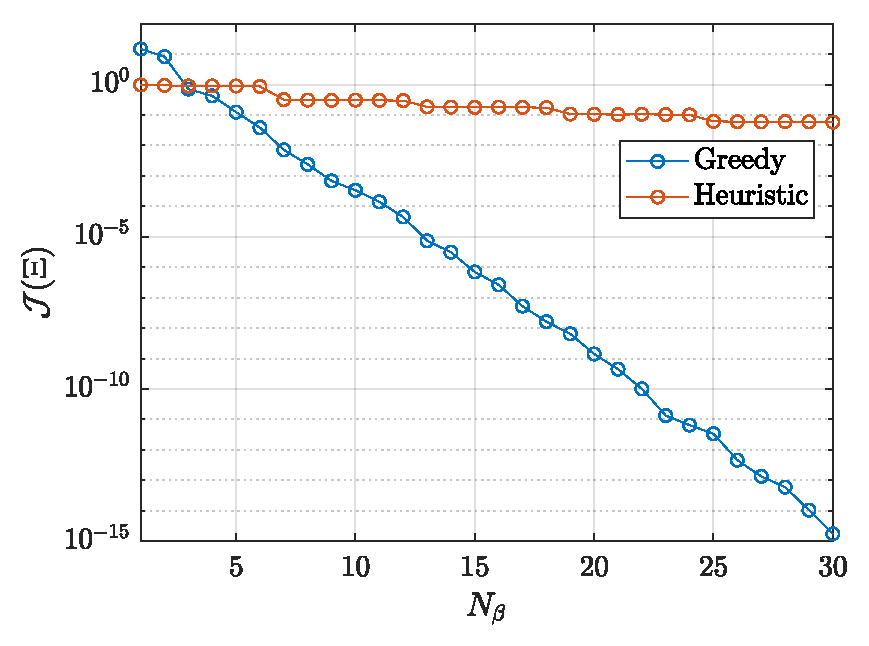
\includegraphics[width=1\linewidth]{figures/Oblique_Obj_P.pdf}
%         \caption{OWNS-P}
%         \label{fig:oblique-obj-p}
%     \end{subfigure}
%     \begin{subfigure}[b]{0.48\textwidth}
%         \centering
%         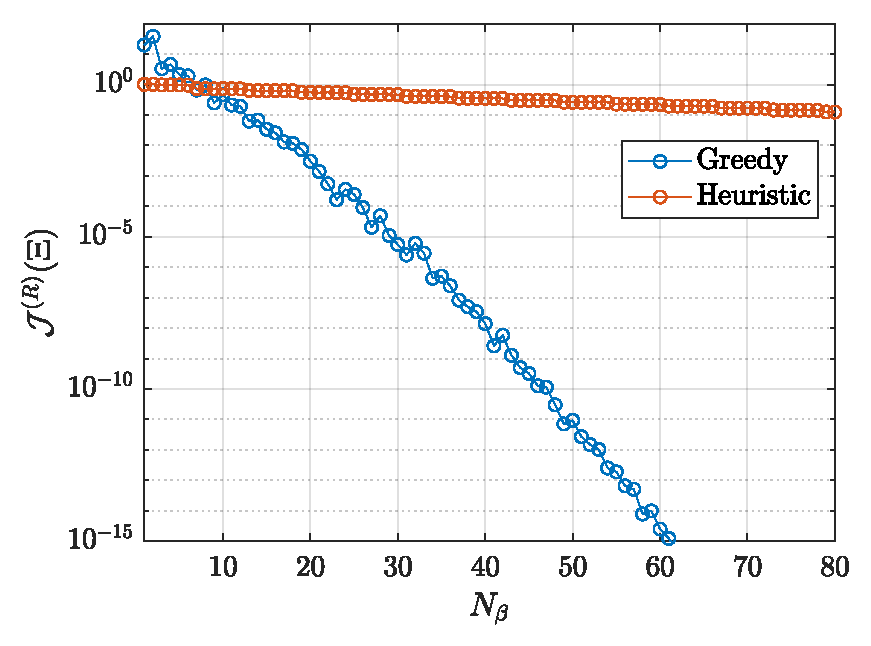
\includegraphics[width=1\linewidth]{figures/Oblique_Obj_R.pdf}
%         \caption{OWNS-R}
%         \label{fig:oblique-obj-r}
%     \end{subfigure}
%     \caption{Objective function convergence for low-speed oblique breakdown.}
%     \label{fig:greedy-converge}
% \end{figure}

\begin{figure}
    \centering
    \begin{subfigure}[b]{0.48\textwidth}
        \centering
        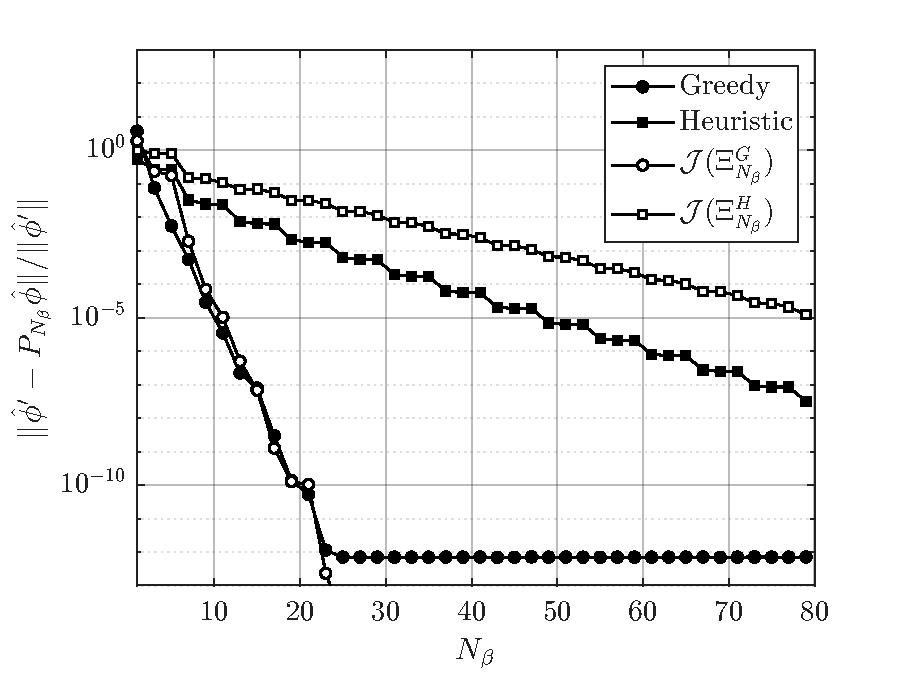
\includegraphics[width=1\linewidth]{figures/Oblique_Err_P_bw.pdf}
        \caption{OWNS-P}\label{fig:oblique-err-p}
    \end{subfigure}
    \begin{subfigure}[b]{0.48\textwidth}
        \centering
        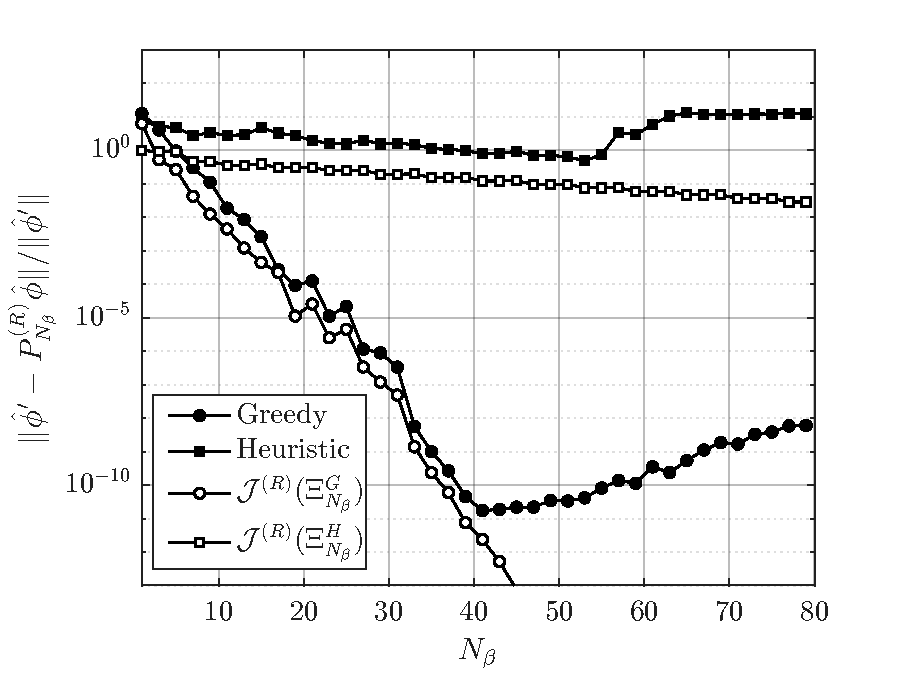
\includegraphics[width=1\linewidth]{figures/Oblique_Err_R_bw.pdf}
        \caption{OWNS-R}\label{fig:oblique-err-r}
    \end{subfigure}\\
    \begin{subfigure}[b]{0.48\textwidth}
        \centering
        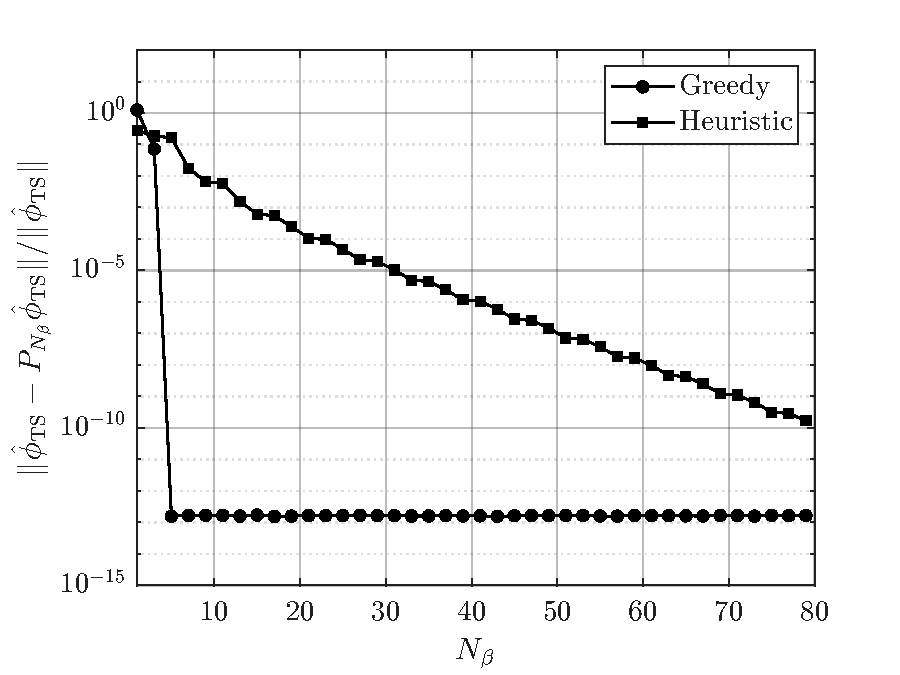
\includegraphics[width=1\linewidth]{figures/Oblique_Err_TS_P_bw.pdf}
        \caption{OWNS-P, TS wave only}\label{fig:oblique-err-TS-p}
    \end{subfigure}
    \begin{subfigure}[b]{0.48\textwidth}
        \centering
        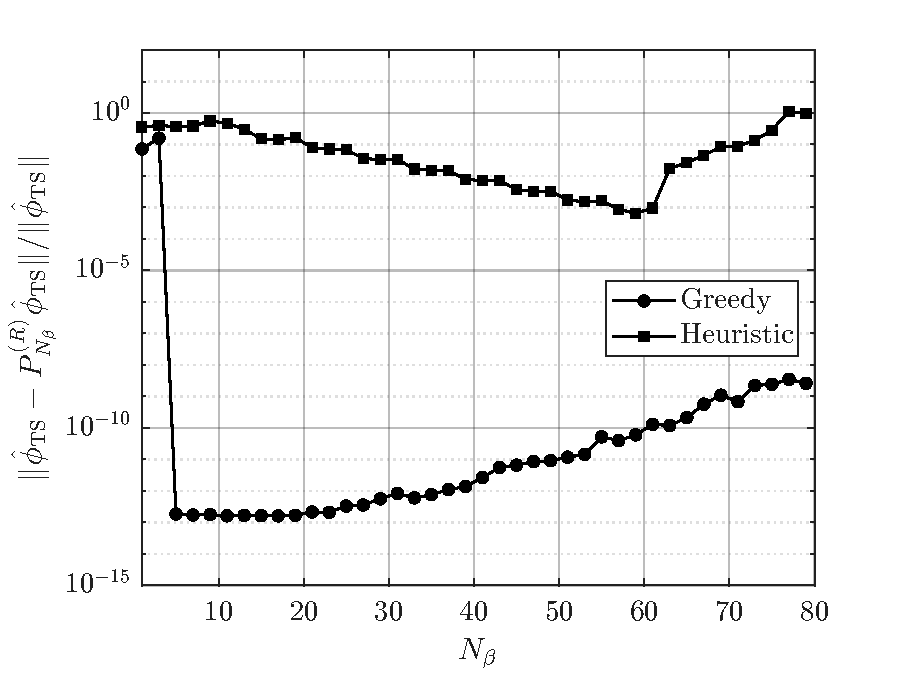
\includegraphics[width=1\linewidth]{figures/Oblique_Err_TS_R_bw.pdf}
        \caption{OWNS-R, TS wave only}\label{fig:oblique-err-TS-r}
    \end{subfigure}\\
    \caption{Error convergence for low-speed oblique breakdown.}
    \label{fig:greedy-err-converge}
\end{figure}

\begin{figure}
    \centering
    \begin{subfigure}[b]{0.48\textwidth}
        \centering
        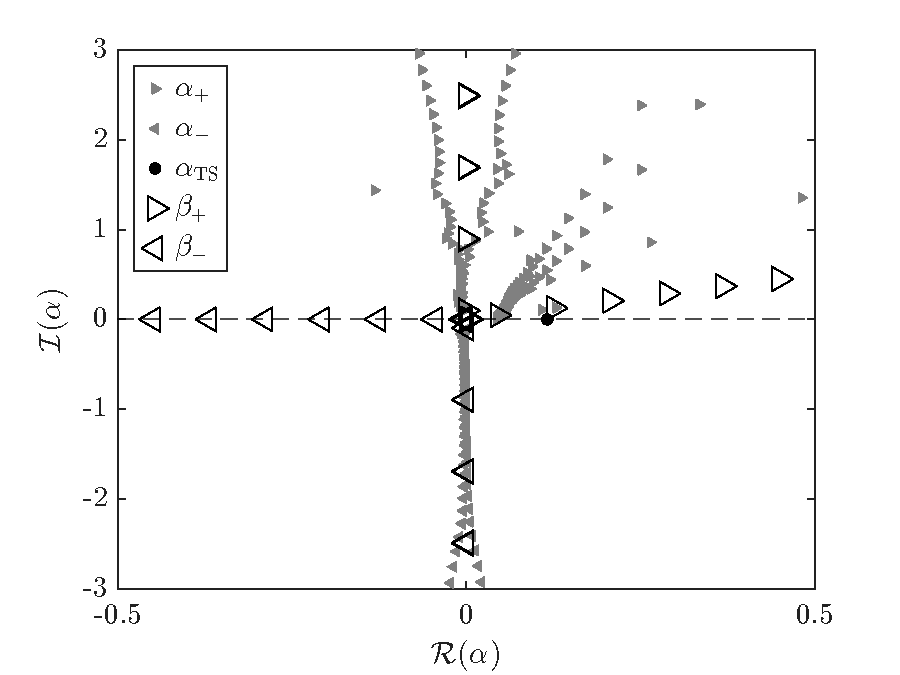
\includegraphics[width=1\linewidth]{figures/Oblique_Params_Heuristic_bw.pdf}
        \caption{Heuristic}
        \label{fig:param-spectrum-heuristic}
    \end{subfigure}
    \begin{subfigure}[b]{0.48\textwidth}
        \centering
        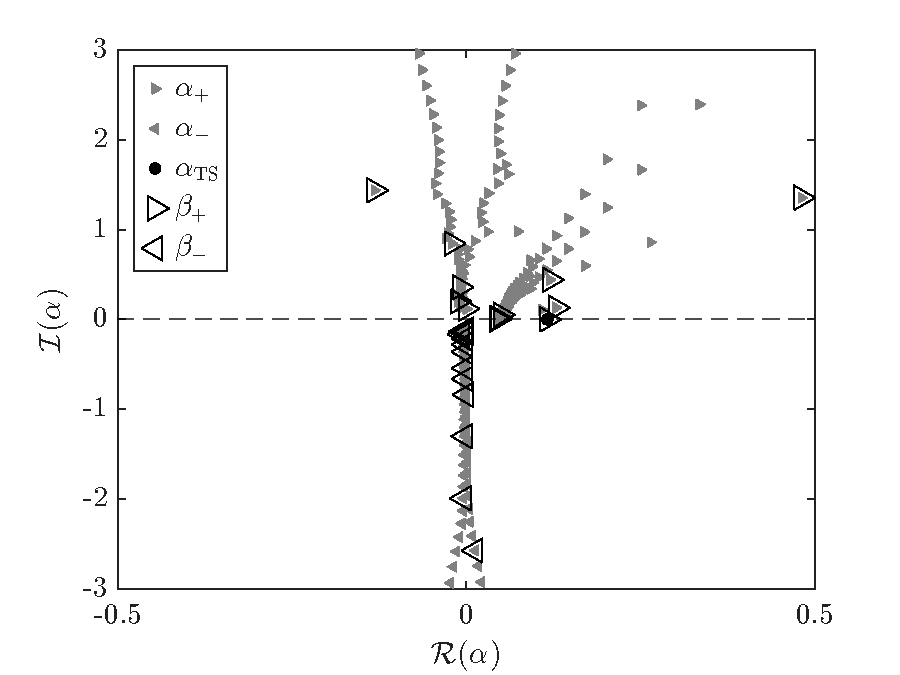
\includegraphics[width=1\linewidth]{figures/Oblique_Params_Greedy_bw.pdf}
        \caption{Greedy}
        \label{fig:param-spectrum-greedy}
    \end{subfigure}
    \caption{Recursion parameters plotted against spectrum for heuristic and greedy recursion parameter selection with $N_\beta = 20$.}
    \label{fig:param-spectrum}
\end{figure}

% Plotting $\hat{\mathcal{J}}_+$ and Figure~\ref{fig:oblique-obj-r-pm} shows that although $\hat{\mathcal{J}}_-$ decreases quickly for heuristic selection, $\hat{\mathcal{J}}_+$ decreases slowly. Since the OWNS-R objective function depends on the maximum value of these two functions, it decreases more slowly than the OWNS-P function. 
% \begin{figure}
%     \centering
%     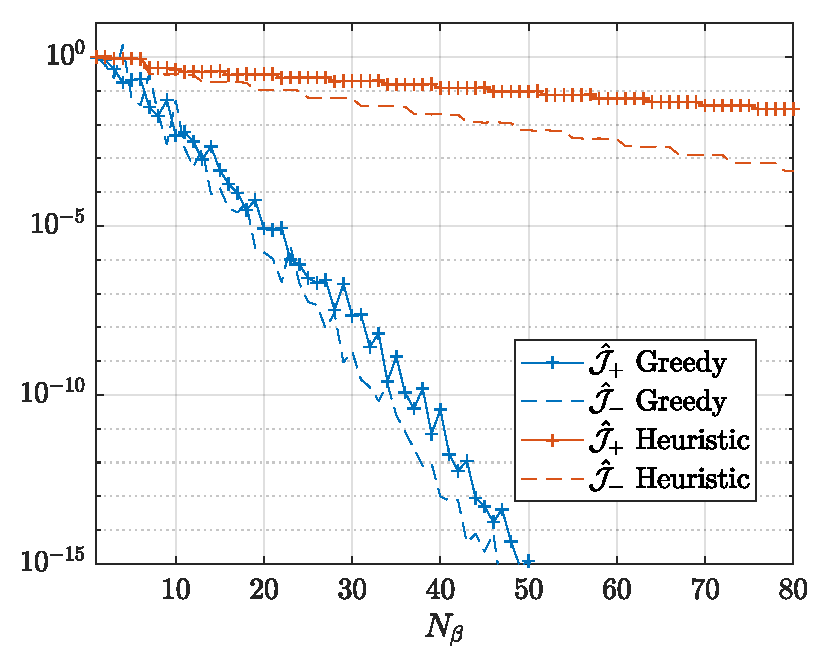
\includegraphics[width=0.48\linewidth]{figures/Oblique_Obj_R_pm.pdf}
%     \caption{Convergence of the objective function, split into left- and right-going components, for greedy and heuristic parameter selection.}
%     \label{fig:oblique-obj-r-pm}
% \end{figure}


\subsection{Stability of the march}\label{subsec:stability}

All left-going modes must be removed for the march to be stable. Figure~\ref{fig:Oblique_OWNS_P_Briggs} shows that heuristic OWNS-P removes all left-going waves from $M$, while Figure~\ref{fig:Oblique_OWNS_R_Briggs} demonstrates that heuristic OWNS-R does not. For $\eta=0$, we observe that the OWNS-R spectrum, $P_{N_\beta}^{(R)}M$, has many eigenvalues with $\mathcal{I}(\alpha)<0$, and taking $\eta=1000$ allows us to verify that these are left-going modes according to Briggs' criterion. This demonstrates that there exists parameter sets for which OWNS-P is stable but OWNS-R is unstable. Repeating this analysis with greedy selection yields stable marches for both OWNS-P and OWNS-R.

% \begin{remark}
% Zhu and Towne~\cite{Zhu_2021_OWNS-R} noted that OWNS-P and OWNS-R approximate the $V$ and $E$, respectively. Therefore, we expect OWNS-P to better remove left-going modes since it makes no approximations to $E$, which is consistent with the above observations.
% \end{remark}

\begin{remark}
Figures 3 and 6 from Zhu and Towne~\cite{Zhu_2021_OWNS-R} show that the OWNS-R operator removes all left-going modes for the dipole and jet test cases, while figure 10 suggests it still supports left-going modes for their supersonic boundary-layer case. Thus, our observations in Figure~\ref{fig:Oblique_OWNS_R_Briggs} are consistent with those of Zhu and Towne~\cite{Zhu_2021_OWNS-R} for their supersonic case.
\end{remark}

\begin{remark}
    In Section~\ref{subsec:OWNSR}, our numerical analysis showed that there exist recursion parameters for which OWNS-P is fully converged while OWNS-R is not (see Proposition~\ref{prop:minimalOWNS-R-false}), which is consistent with our observations in Figure~\ref{fig:greedy-stability}.
\end{remark}

\begin{figure}
    \centering
    \begin{subfigure}[b]{0.48\textwidth}
        \centering
        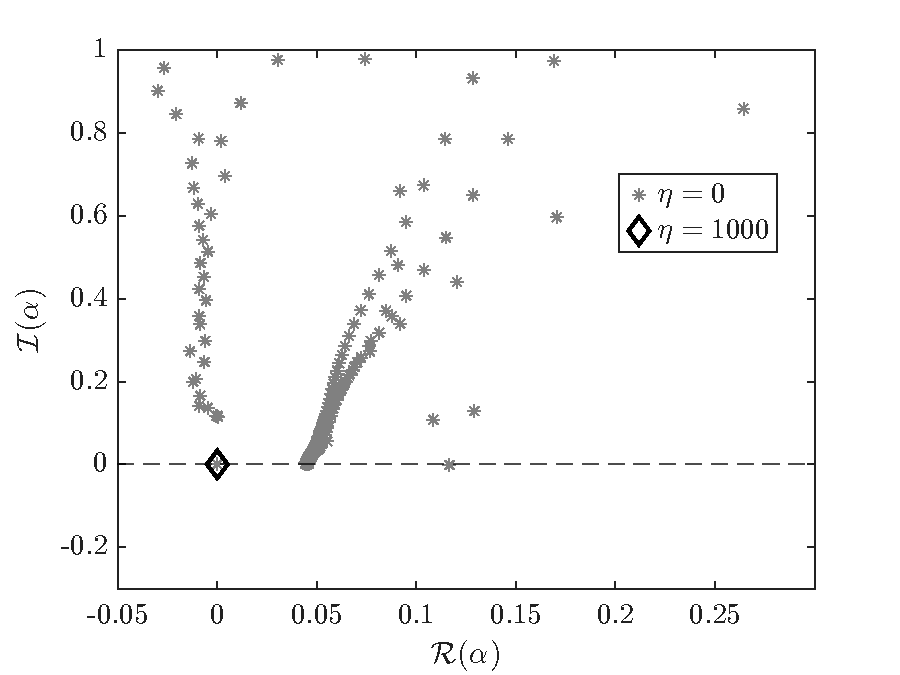
\includegraphics[width=1\linewidth]{figures/Oblique_OWNS_P_Briggs_bw.pdf}
        \caption{Heuristic OWNS-P, $N_\beta=15$}\label{fig:Oblique_OWNS_P_Briggs}
    \end{subfigure}
    \begin{subfigure}[b]{0.48\textwidth}
        \centering
        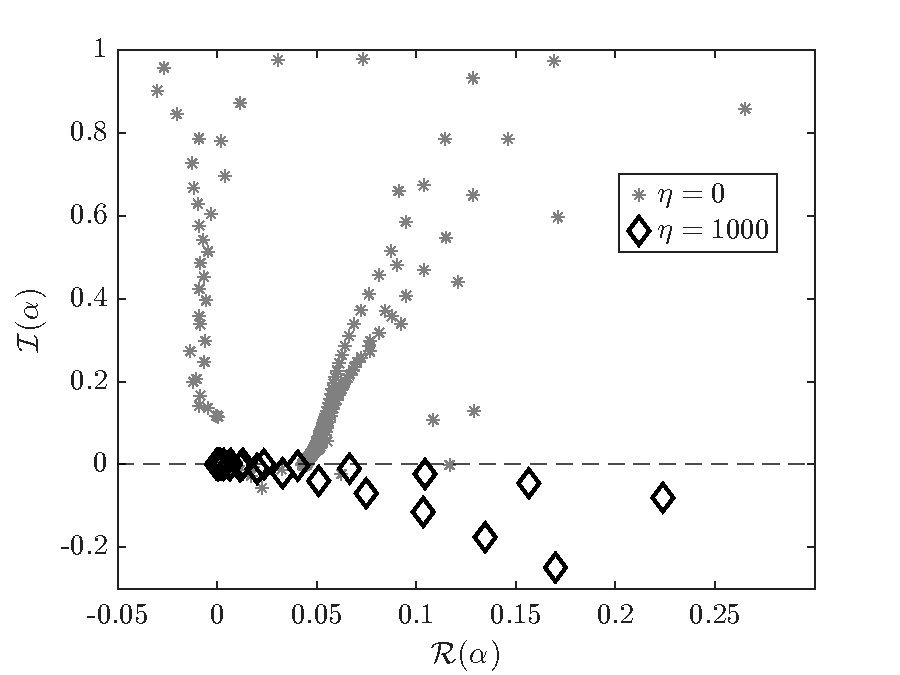
\includegraphics[width=1\linewidth]{figures/Oblique_OWNS_R_Briggs_bw.pdf}
        \caption{Heuristic OWNS-R, $N_\beta=52$}\label{fig:Oblique_OWNS_R_Briggs}
    \end{subfigure}\\
    \caption{For the march to be stable, the OWNS spectrum ($P_{N_\beta}M$) must not support any left-going modes. According to Briggs' criterion, a mode is left-going if $\mathcal{I}(\alpha)<0$ as $\eta\to\infty$. Figure~\ref{fig:Oblique_OWNS_P_Briggs} shows that heuristic OWNS-P does not have $\mathcal{I}(\alpha)<0$ for $\eta=1000$, while~\ref{fig:Oblique_OWNS_R_Briggs} shows that heuristic OWNS-R does, so that the heuristic OWNS-R march is unstable.}
    \label{fig:greedy-stability}
\end{figure}


% \begin{figure}
%     \centering
%     \begin{subfigure}[b]{0.48\textwidth}
%         \centering
%         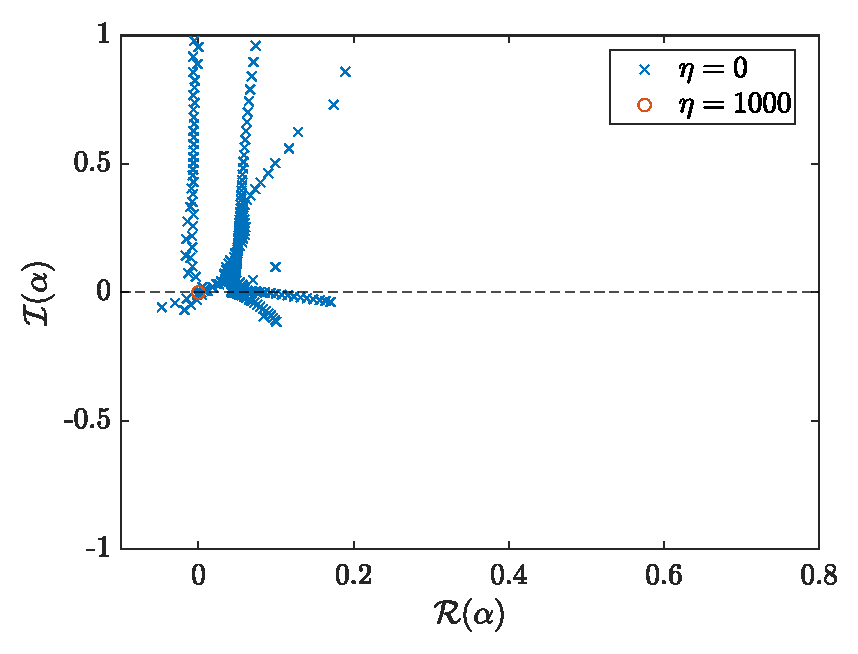
\includegraphics[width=1\linewidth]{figures/Bertolotti_OWNS_P_Briggs_03.pdf}
%         \caption{OWNS-P, $N_\beta=3$}\label{fig:Bertolotti_OWNS_P_Briggs_03}
%     \end{subfigure}
%     \begin{subfigure}[b]{0.48\textwidth}
%         \centering
%         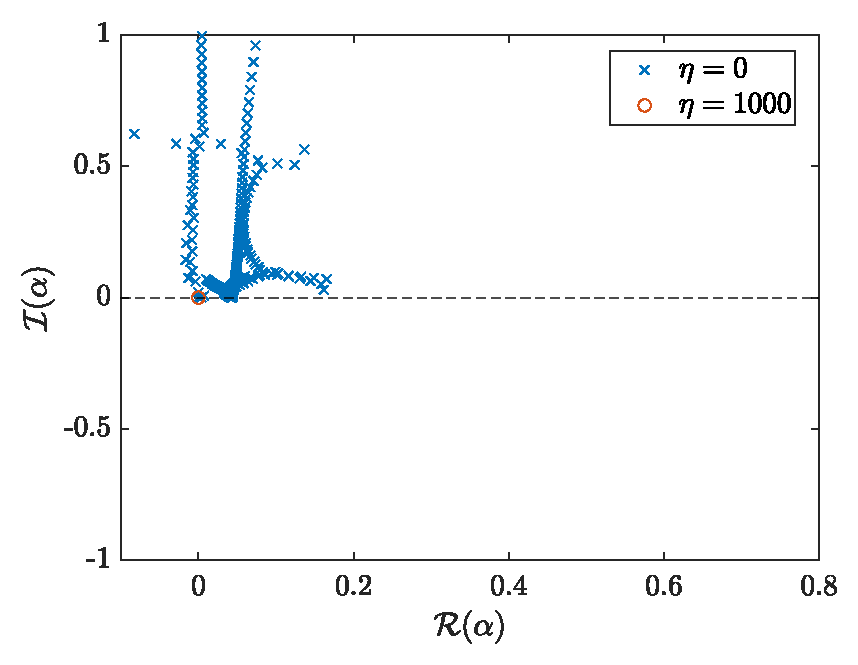
\includegraphics[width=1\linewidth]{figures/Bertolotti_OWNS_P_Briggs_06.pdf}
%         \caption{OWNS-R, $N_\beta=6$}\label{fig:Bertolotti_OWNS_P_Briggs_06}
%     \end{subfigure}\\
%     \caption{Comparison of OWNS-P spectrum using heuristic parameter selection for $\eta=0$ and $\eta=1000$. According to Briggs' criterion, $\mathcal{I}(\alpha)<0$ for large values of $\eta$ indicates a right-going mode. For $\eta=0$, we wish to have $\mathcal{I}(\alpha)\geq0$ for the march to be stable. We achieve a stable march using OWNS-P and with both $N_\beta=3$ and $N_\beta=6$, because there are no left-going modes, according to Briggs' criterion.}
%     \label{fig:Bertolotti_OWNS_P_Briggs_compare}
% \end{figure}


%\subsubsection{Accuracy of the right-going eigenvalues}

%To further assess the performance of the recursion parameters, we plot the spectrum of $P_{N_\beta}M$ against that of $M$ for heuristic and greedy parameter selection in figure~\ref{fig:OWNS-spectrum-compare}. The greedy parameter selection properly tracks right-going modes for large values of $\mathcal{I}(\alpha)>0$, while heuristic parameter selection does not. Similarly, the greedy parameter selection properly tracks right-going vortical modes for $\mathcal{R}(\alpha)\in[0.042,0.044]$ and $\mathcal{I}(\alpha)\in(0,0.04)$, while heuristic parameter selection does not. However, most importantly, both greedy and heuristic parameter remove left-going waves and properly evolve track the TS wave, which explains why heuristic parameter selection works well in practice for OWNS-P. We make a similar comparison for OWNS-R in figure~\ref{fig:OWNS-R-spectrum-compare}, where we observe that the heuristic approach fares far worse for OWNS-R than OWNS-P, while the greedy approach works reasonably well. We note that the greedy approach for OWNS-R requires far more recursion parmaeters for accuracy and stability compared to OWNS-P.

% \begin{figure}
%     \centering
%     \begin{subfigure}[b]{0.48\textwidth}
%         \centering
%         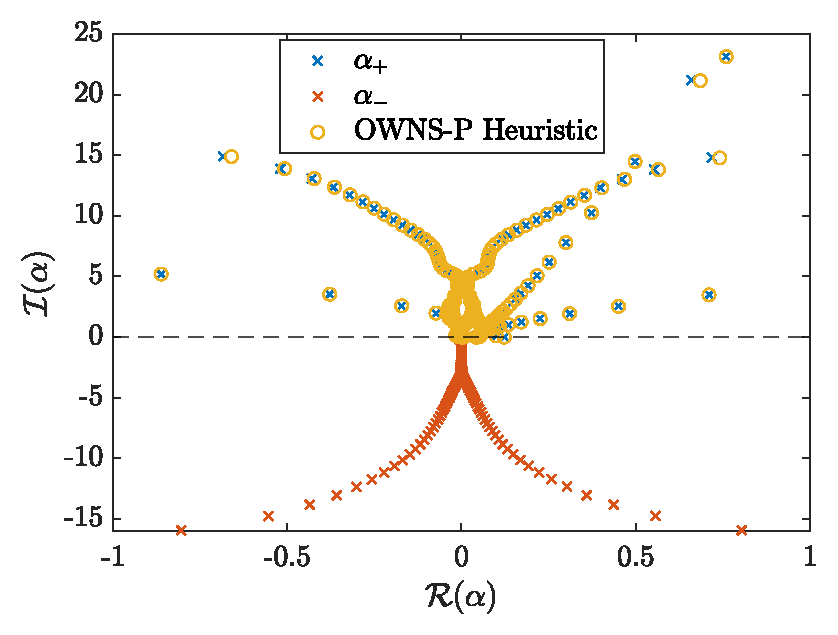
\includegraphics[width=1\linewidth]{figures/Bertolotti_OWNS_Spectrum_Heuristic.pdf}
%     \end{subfigure}
%     \begin{subfigure}[b]{0.48\textwidth}
%         \centering
%         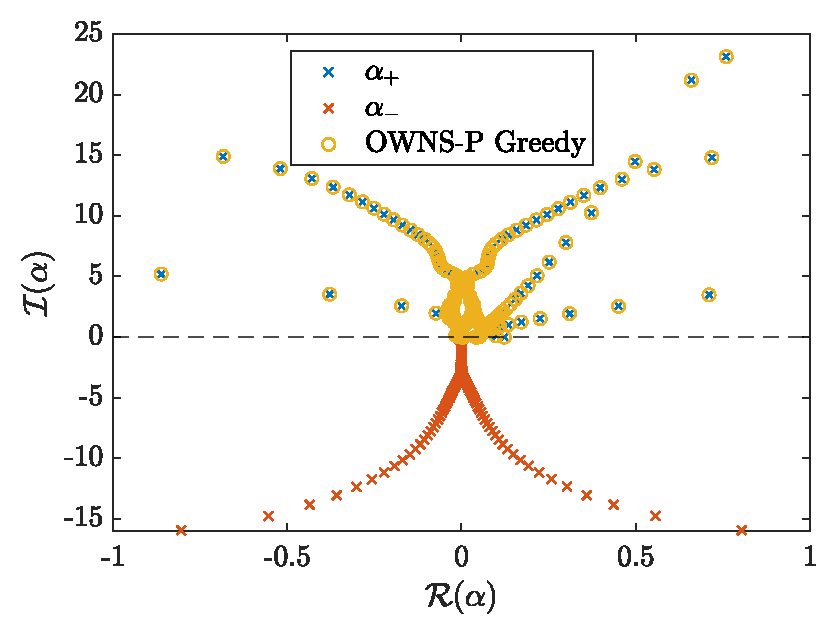
\includegraphics[width=1\linewidth]{figures/Bertolotti_OWNS_Spectrum_Greedy.pdf}
%     \end{subfigure}\\
%     \begin{subfigure}[b]{0.48\textwidth}
%         \centering
%         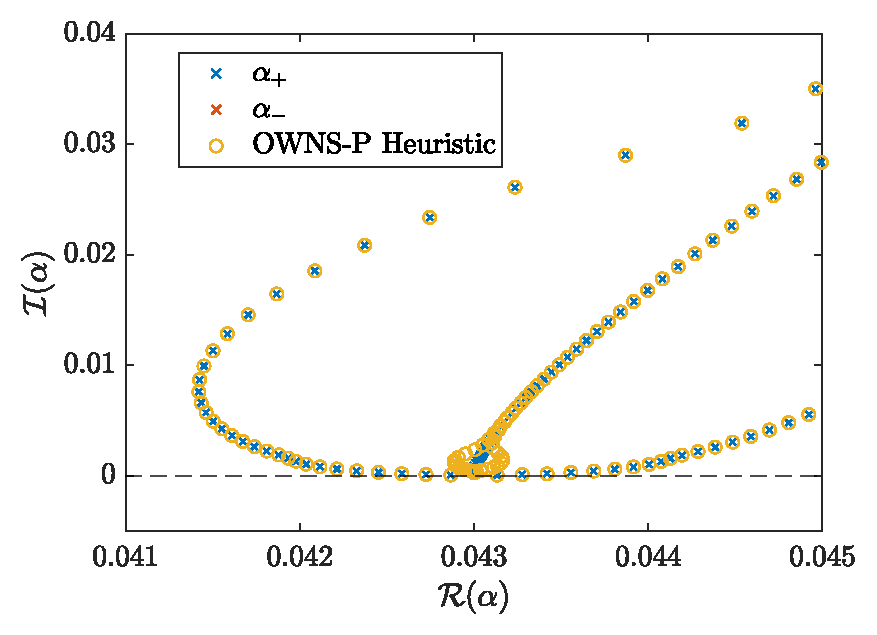
\includegraphics[width=1\linewidth]{figures/Bertolotti_OWNS_Spectrum_Zoom_Heuristic.pdf}
%     \end{subfigure}
%     \begin{subfigure}[b]{0.48\textwidth}
%         \centering
%         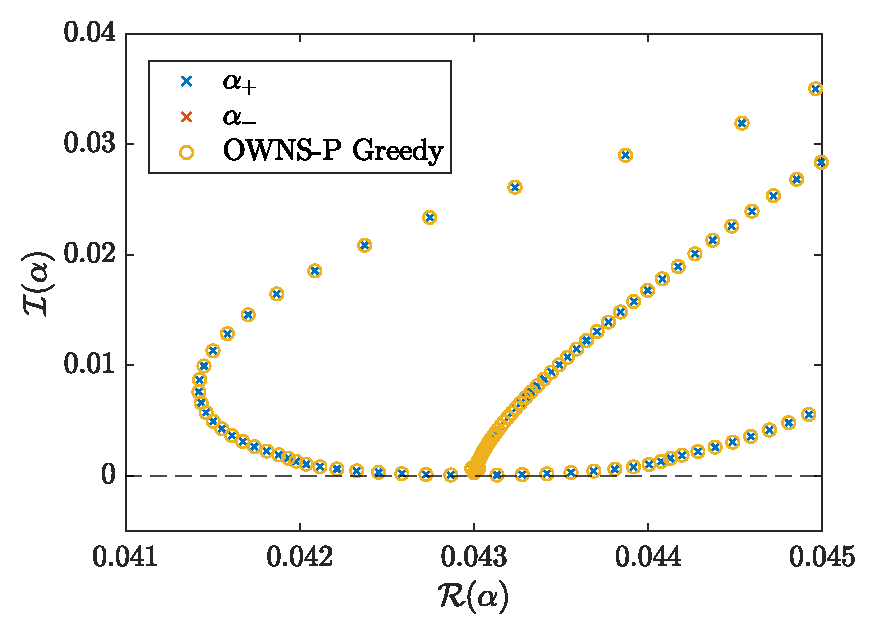
\includegraphics[width=1\linewidth]{figures/Bertolotti_OWNS_Spectrum_Zoom_Greedy.pdf}
%     \end{subfigure}
%     \caption{Comparison of the spectrum of $M$ against $P_{N_\beta}M$ for heuristic and greedy parameter selection.}
%     \label{fig:OWNS-spectrum-compare}
% \end{figure}

% \begin{figure}
%     \centering
%     \begin{subfigure}[b]{0.48\textwidth}
%         \centering
%         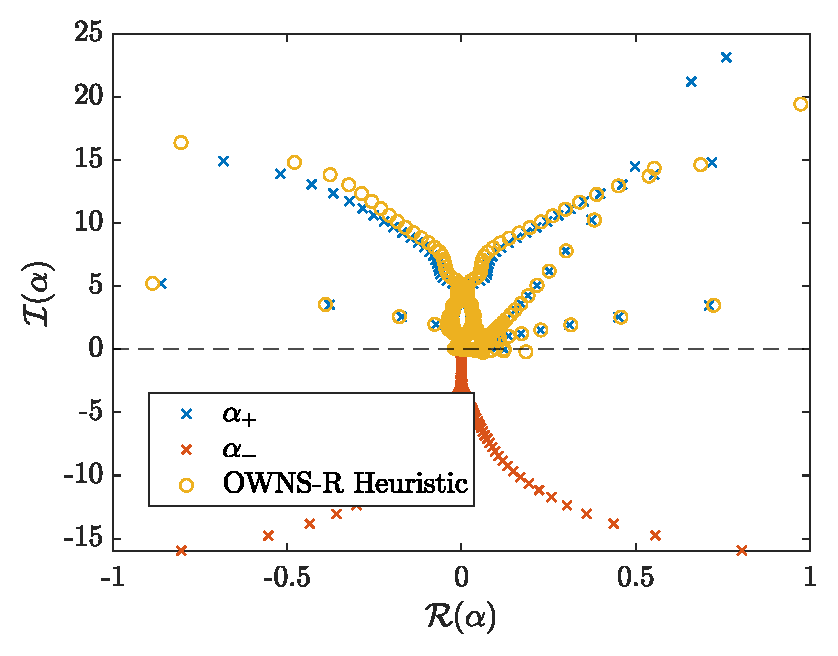
\includegraphics[width=1\linewidth]{figures/Bertolotti_OWNS_R_Spectrum_Heuristic.pdf}
%     \end{subfigure}
%     \begin{subfigure}[b]{0.48\textwidth}
%         \centering
%         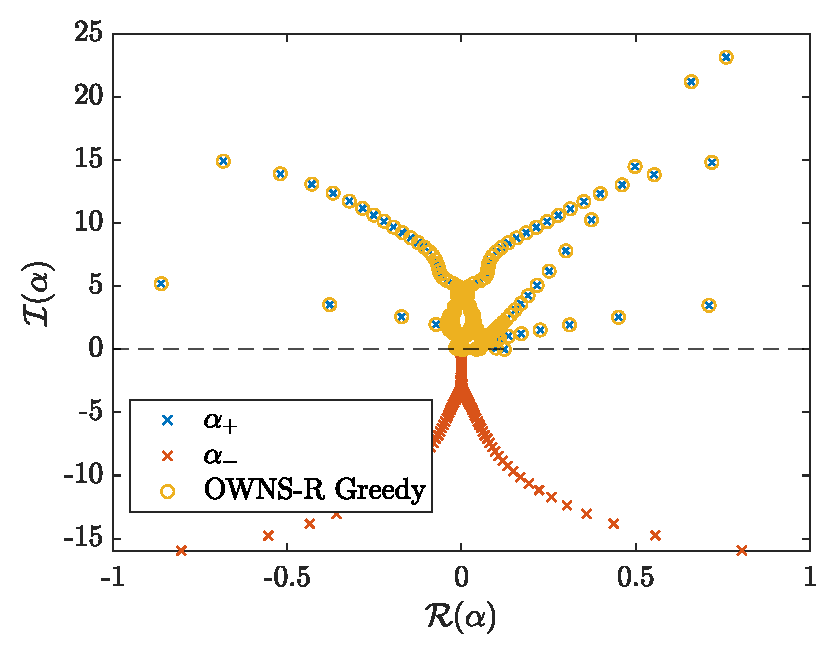
\includegraphics[width=1\linewidth]{figures/Bertolotti_OWNS_R_Spectrum_Greedy.pdf}
%     \end{subfigure}\\
%     \begin{subfigure}[b]{0.48\textwidth}
%         \centering
%         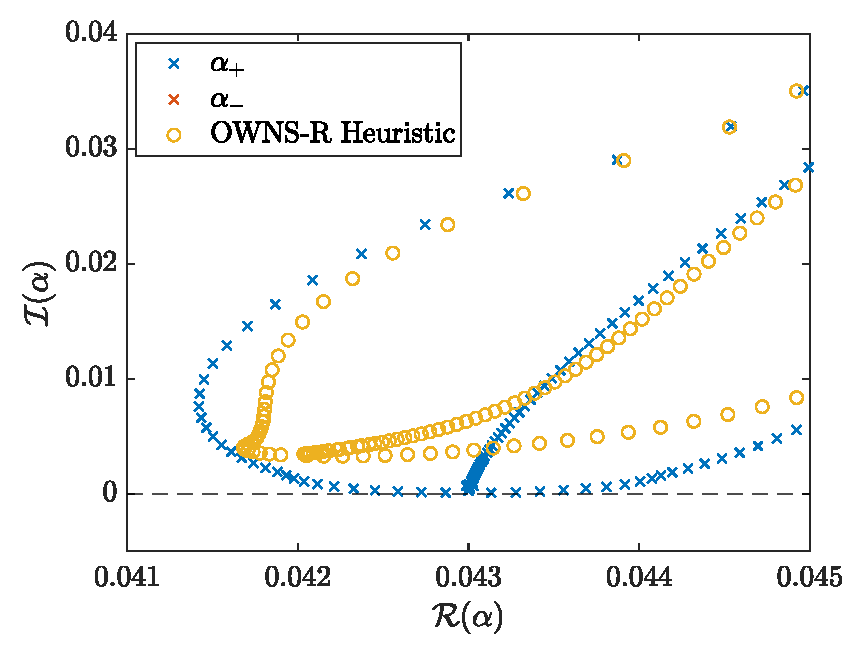
\includegraphics[width=1\linewidth]{figures/Bertolotti_OWNS_R_Spectrum_Zoom_Heuristic.pdf}
%     \end{subfigure}
%     \begin{subfigure}[b]{0.48\textwidth}
%         \centering
%         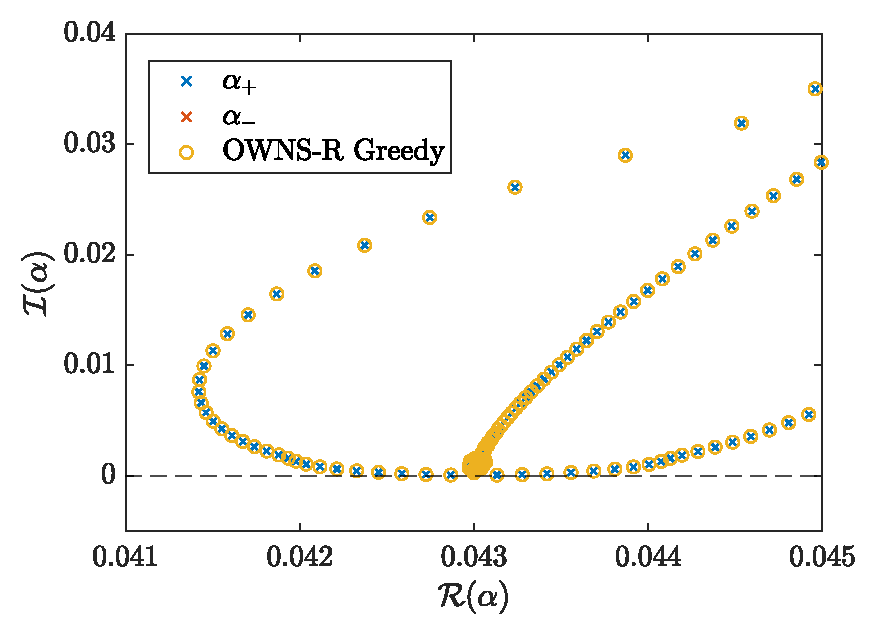
\includegraphics[width=1\linewidth]{figures/Bertolotti_OWNS_R_Spectrum_Zoom_Greedy.pdf}
%     \end{subfigure}
%     \caption{Comparison of the spectrum of $M$ against $P_{N_\beta}^{(R)}M$ for heuristic and greedy parameter selection.}
%     \label{fig:OWNS-R-spectrum-compare}
% \end{figure}


% \subsection{Comparison for different flows}

% We expand our discussion to include a 3D low-speed boundary-layer flow and a 2D high-speed boundary-layer flow.

% \subsubsection{3D low-speed boundary-layer flow}~\label{sec:joslin}

% We investigate the oblique-wave case studied by Joslin et al.~\cite{Joslin_1993_DNS} for a low-speed isothermal flat plate boundary-layer flow with disturbance frequency and wavenumber are $F = 86 \times 10^{-6}$ and $b = 0.222 \times 10^{-3}$, respectively, for the wall-normal domain $y\in[0,60]$ with $N_y=100$ at $Re_x=2.74\times10^5$. Figure~\ref{fig:oblique-err} shows that greedy selection yields rapid convergence of the objective function and projection error. Moreover, OWNS-P achieves machine-zero error with $N_\beta=24$, while OWNS-R does not, due to rounding errors in computing $\beta_*^j$. We further note that the 3D case converges with fewer recursion parameters because the left- and right-going branches are more widely separated than in the 2D case, which makes it easier to choose recursion parameters that keep both $\|F_{++}\|$ and $\|F_{--}^{-1}\|$ small, as noted by Towne and Colonius~\cite{Towne_2015_OWNS-O}.


% \begin{figure}
%     \centering
%     \begin{subfigure}[b]{0.48\textwidth}
%         \centering
%         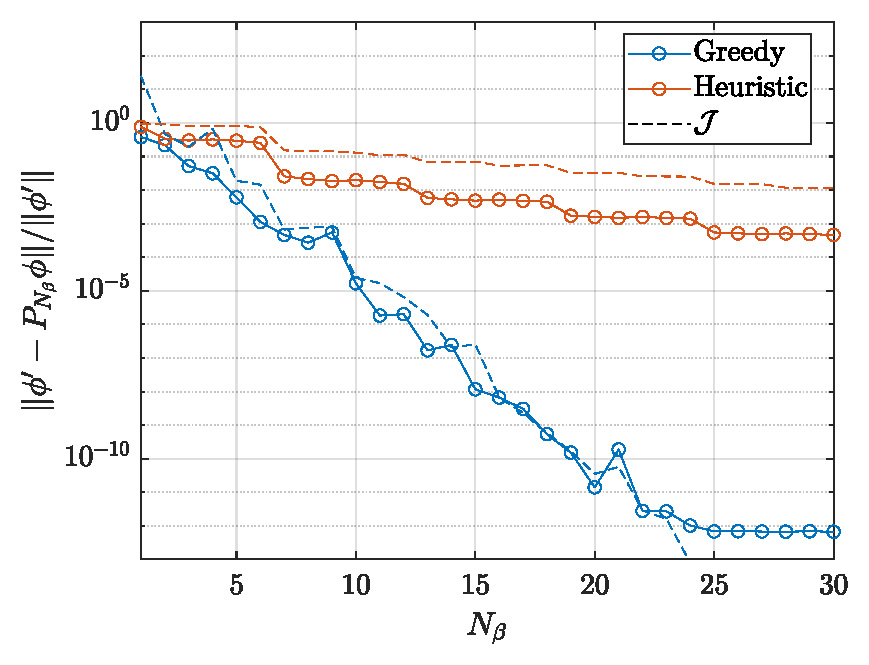
\includegraphics[width=1\linewidth]{figures/Oblique_Err_Obj_P.pdf}
%         \caption{OWNS-P}\label{fig:oblique-err-p}
%     \end{subfigure}
%     \begin{subfigure}[b]{0.48\textwidth}
%         \centering
%         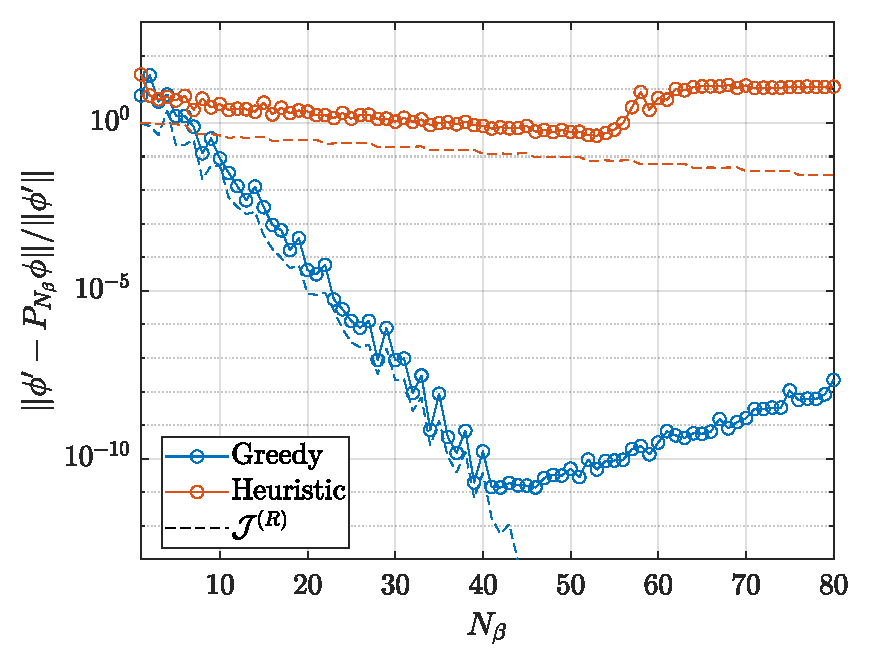
\includegraphics[width=1\linewidth]{figures/Oblique_Err_Obj_R.pdf}
%         \caption{OWNS-R}\label{fig:oblique-err-r}
%     \end{subfigure}
%     \caption{Error convergence as a function of $N_\beta$ for OWNS-P and OWNS-R for the low-speed oblique wave case.}
%     \label{fig:oblique-err}
% \end{figure}


% \subsubsection{2D high-speed boundary-layer flow}~\label{sec:zhong}

% We consider the Mach 4.5 boundary-layer flow over an adiabatic flat plate studied by Ma and Zhong~\cite{Ma_2003_DNS_1}, which was used by Zhu and Towne~\cite{Zhu_2021_OWNS-R} as a validation case for the OWNS-R formulation. The flow conditions are $M_\infty = 4.5$, $T_\infty^*=65.15$ K, $p_\infty^*=728.44$ Pa, $Pr=0.72$, and unit Reynolds number $Re_\infty^* = \rho_\infty^* U_\infty^* / \mu_\infty^*=7.2\times10^6 / $ m. We compare the greedy and heuristic approaches at $Re_x=5.625\times10^3$, and figure~\ref{fig:zhong-err} shows the convergence of the error as a function of $N_\beta$ for OWNS-P and OWNS-R. We again observe that OWNS-P achieves machine zero error, while OWNS-R does not. For OWNS-R only, we have excluded right-going eigenvalues with $\alpha_i>100$ from the greedy selection procedure, which improves the accuracy of the approximation, since these modes decay rapidly. We also note that heuristic selection is better at evolving Mack's second mode (MM), which is the dominant instability for high-speed boundary-layer flows, as the they have been clustered near it for better accuracy~\cite{Kamal_2023_Thesis}.

% \begin{figure}
%     \centering
%     \begin{subfigure}[b]{0.48\textwidth}
%         \centering
%         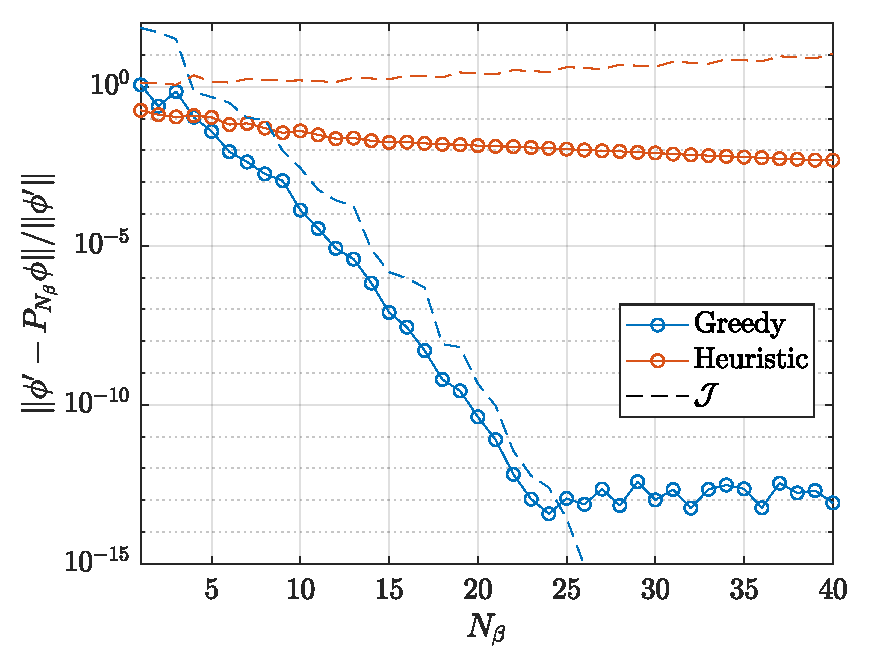
\includegraphics[width=1\linewidth]{figures/Zhong-OWNS-P.pdf}
%         \caption{OWNS-P}
%         \label{fig:zhong-err-p}
%     \end{subfigure}
%     \begin{subfigure}[b]{0.48\textwidth}
%         \centering
%         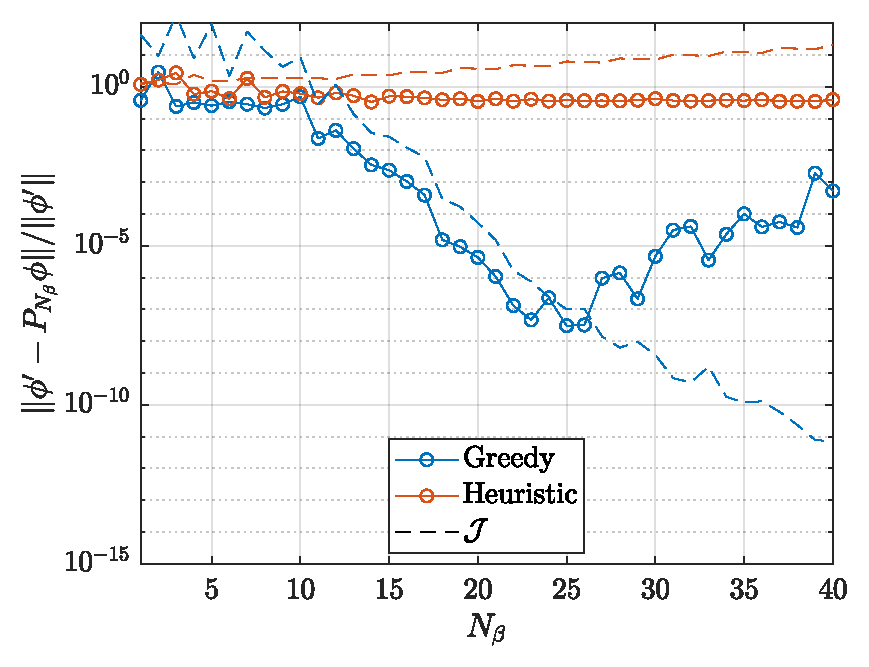
\includegraphics[width=1\linewidth]{figures/Zhong-OWNS-R.pdf}
%         \caption{OWNS-R}
%         \label{fig:zhong-err-r}
%     \end{subfigure}\\
%     \begin{subfigure}[b]{0.48\textwidth}
%         \centering
%         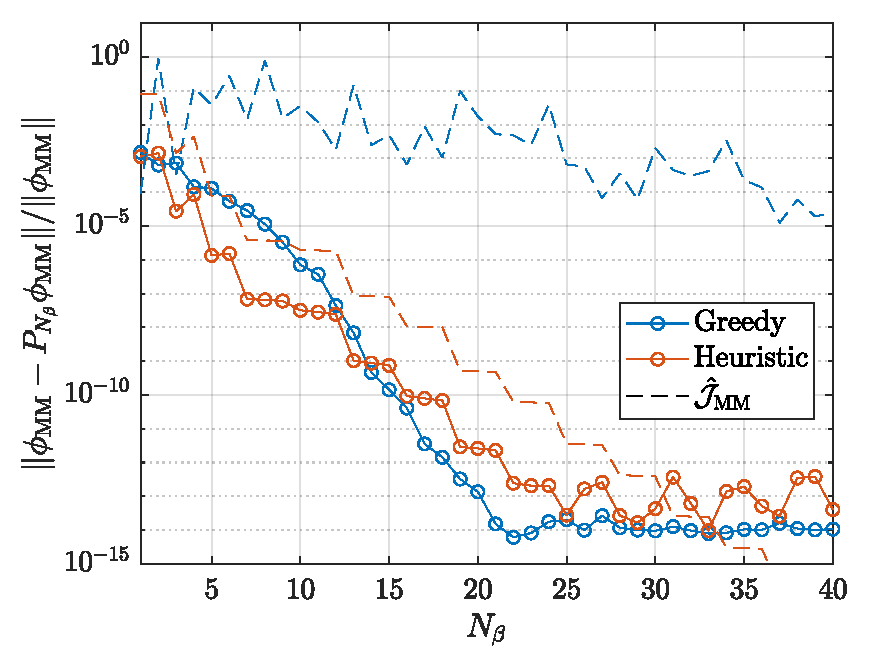
\includegraphics[width=1\linewidth]{figures/Zhong-OWNS-P-MM.pdf}
%         \caption{OWNS-P, MM only}
%         \label{fig:zhong-err-p-MM}
%     \end{subfigure}
%     \begin{subfigure}[b]{0.48\textwidth}
%         \centering
%         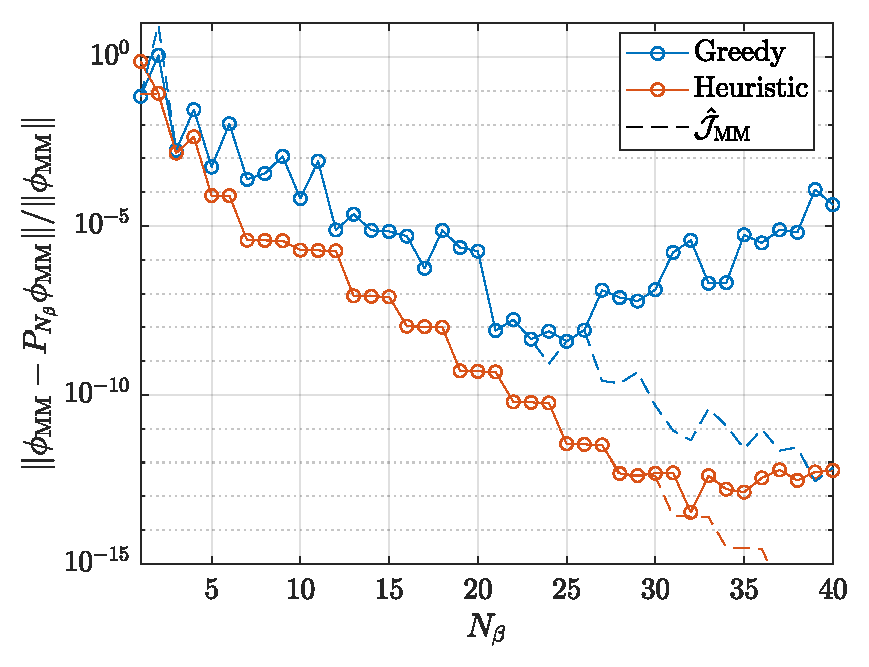
\includegraphics[width=1\linewidth]{figures/Zhong-OWNS-R-MM.pdf}
%         \caption{OWNS-R, MM only}
%         \label{fig:zhong-err-r-MM}
%     \end{subfigure}
%     \caption{Convergence of the error for greedy and heuristic parameter selection for 2D high-speed boundary-layer flow.}
%     \label{fig:zhong-err}
% \end{figure}


\section{Demonstration of the greedy algorithm for spatial marching}\label{sec:greedyMarching}

Here we demonstrate that although the greedy algorithm must compute the eigenvalues of $M$, it leads to a net decrease in computational cost for linear and nonlinear disturbance evolution in low- and high-speed boundary-layer flows. In addition, we show that greedy selection alleviates numerical errors introduced by heuristic parameter selection for nonlinear disturbance evolution in a high-speed boundary-layer flow.


\subsection{3D low-speed oblique breakdown}

We first demonstrate for the  oblique breakdown case discussed in Section~\ref{sec:greedySingle} that greedy parameter selection reduces computational cost in both linear and nonlinear calculations. The problem parameters remain the same as before, and we consider the streamwise domain $Re_x \in [2.74, 6.08] \times 10^5$ with $N_x=2000$ stations. We compare the number of recursion parameters required for convergence of the relative error in the $N$-factor, which is a measure of the disturbance growth used in the $e^N$ method to empirically predict laminar-turbulent transition in boundary-layer flows~\cite{VanIngen_1956_eN,Smith_1956_eN}, and measure speed-up based on total wall-clock time. Note that the $N$-factor is defined as $N = \max_{x} \ln [ A(x) / A(x_0) ]$, where $A(x) = \max_{y} u'(x,y)$ is the disturbance amplitude and $x_0$ is domain inlet.


\subsubsection{Linear calculation}

OWNS-R with heuristic parameter selection does not remove left-going waves, so the march is unstable (see Section~\ref{subsec:stability}). Therefore, we compare OWNS-P and OWNS-R using greedy selection against OWNS-P using heuristic selection. To make meaningful comparisons, we take $N_\beta$ to be the smallest value that yields 10\%, 1\%, and 0.1\% relative error in the $N$-factor, measured against greedy OWNS-P with $N_\beta = 30$. Table~\ref{tab:oblique-lin-err} shows that greedy selection leads to a speed-up for both OWNS-R and OWNS-P, and that this speed-up pronounced for OWNS-R at 1\% error and OWNS-P and 0.1\% error.

\begin{table}
    \centering
    \begin{tabular}{ c | c c c | c c c }
              & & $N_\beta$ & & & Speed-up &\\
        Error & P-H & P-G & R-G & P-H & P-G & R-G\\ \hline
        10\%  & 11  & 5   & 29  & 1.0 & 2.3 & 3.6\\ \hline
        1\%   & 17  & 5   & 29  & 1.0 & 3.9 & 6.0\\ \hline
        0.1\% & 18  & 5   & 36  & 1.0 & 4.2 & 4.9
    \end{tabular}
    \caption{Speed-up achieved using greedy selection with OWNS-P (P-G) and OWNS-R (R-G) relative to heuristic selection with OWNS-P (P-H) for 3D low-speed oblique-wave breakdown.}
    \label{tab:oblique-lin-err}
\end{table}


\subsubsection{Nonlinear calculation}

For the nonlinear calculations, we truncate the Fourier series at $M=3$ temporal and $N=4$ spanwise modes, while we specify at the inlet that the oblique wave has amplitude 0.141\% based on the free-stream $u$-velocity. We select $N_\beta$ to be the smallest value such that the relative error in the $N$-factor is 0.1\% with respect to the reference solution (greedy selection with $N_\beta=30$). For NOWNS, heuristic and greedy parameter selection require $N_\beta = 18$ and $N_\beta = 6$, respectively, resulting in a speed-up of 3.83 for the greedy approach. 

% Figure~\ref{fig:oblique-nowns} compares solutions obtained using NOWNS with $N_\beta=6$ for greedy and heuristic selection, and shows that heuristic selection leads to solution blow-up, while greedy does not.

% \begin{figure}
%     \centering
%     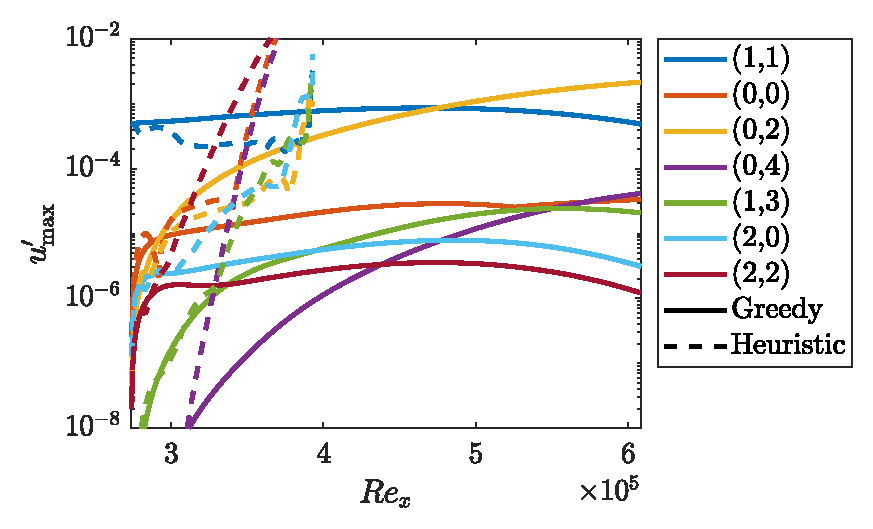
\includegraphics[width=0.7\linewidth]{figures/Oblique_NOWNS.pdf}
%     \caption{NOWNS for oblique-wave breakdown, comparing greedy and heuristic recursion parameter selection with $N_\beta=6$. Although NOWNS with greedy selection is sufficiently converged, heuristic selection is not, and the solution blows-up.}
%     \label{fig:oblique-nowns}
% \end{figure}

% \subsubsection{Linear calculation}

% We compute the $N$-factor based on the temperature, rather than velocity, disturbance and take the reference solution to be the greedy OWNS-P calculation with $N_\beta=20$. Table~\ref{tab:oblique-lin-MM-err} shows that heuristic recursion parameter selection generally converges faster than greedy, consistent with our observation in section~\ref{sec:zhong} that the error in Mack's second mode converges faster using heuristic selection. For linear calculations dominated by Mack's second mode, heuristic selection may be preferable. However, greedy selection may perform better for more complicated calculations involving more eigenvectors of $M$, which we demonstrate for our nonlinear calculation.

% \begin{table}
%     \centering
%     \begin{tabular}{ c | c c c | c c c }
%               & & $N_\beta$ & & & Speed-up &\\
%         Error & P-H & P-G & R-G & P-H & P-G & R-G\\ \hline
%         10\%  & 1  & 6   & 17  & 1.0 & 0.34 & 0.83\\ \hline
%         1\%   & 1  & 6   & 21  & 1.0 & 0.34 & 0.83\\ \hline
%         0.1\% & 2  & 7   & 22  & 1.0 & 0.32 & 0.82
%     \end{tabular}
%     \caption{Speed-up achieved by using greedy parameter selection with OWNS-P (P-G) and OWNS-R (R-G) relative to heuristic parameter selection with OWNS-P (P-H) for different relative errors in the $N$-factor for the 2D high-speed boundary-layer flow.}
%     \label{tab:oblique-lin-MM-err}
% \end{table}


% \subsubsection{Nonlinear calculation}

\subsection{2D high-speed Mack's second mode}

We apply NOWNS to the Mach 4.5 boundary-layer flow over an adiabatic flat plate studied by Ma and Zhong~\cite{Ma_2003_DNS_1}, where $M_\infty = 4.5$, $T_\infty^*=65.15$ K, $p_\infty^*=728.44$ Pa, $Pr=0.72$, and $Re_\infty^* = \rho_\infty^* U_\infty^* / \mu_\infty^*=7.2\times10^6 / $ m. For the disturbance frequency $F=2.2\times10^{-4}$, Mack's second mode (MM) is the dominant instability. We truncate the Fourier series at $M=10$ modes and specify that MM have an amplitude of 10\% based on the free-stream temperature. We compare the temperature profiles obtained using greedy and heuristic parameter selection in Figure~\ref{fig:NOWNS-Zhu-01}, and discuss how heuristic NOWNS introduces spurious numerical fluctuations along the sonic line.

Figure~\ref{fig:NOWNS-Zhu-T1-0500} shows that greedy and heuristic parameter selection predict similar temperature profiles for $T_1'$ near the inlet, while Figure~\ref{fig:NOWNS-Zhu-T1-2501} shows that at the domain outlet, heuristic NOWNS predicts a feature along the sonic line that is not predicted by greedy NOWNS. Figure~\ref{fig:NOWNS-Zhu-T3-0500} shows that near the domain inlet, heuristic NOWNS predicts a large fluctuation in $T_3'$ that is not predicted by greedy NOWNS. As the solution is marched downstream, this feature corrupts the solution, eventually leading to the fluctuation in $T_1'$ observed for heuristic NOWNS in Figure~\ref{fig:NOWNS-Zhu-T1-2501}. Although $T_1'$ is similar between the greedy and heuristic NOWNS calculations at the domain outlet, Figure~\ref{fig:NOWNS-Zhu-T3-2501} shows that $T_3'$ is substantially different, which corrupts the evolution of $T_1'$ in heuristic NOWNS. We note that although we plot only $T_3'$, similar results are observed for the other harmonics of $T_1'$.

\begin{figure}
    \centering
    \begin{subfigure}[b]{0.48\textwidth}
        \centering
        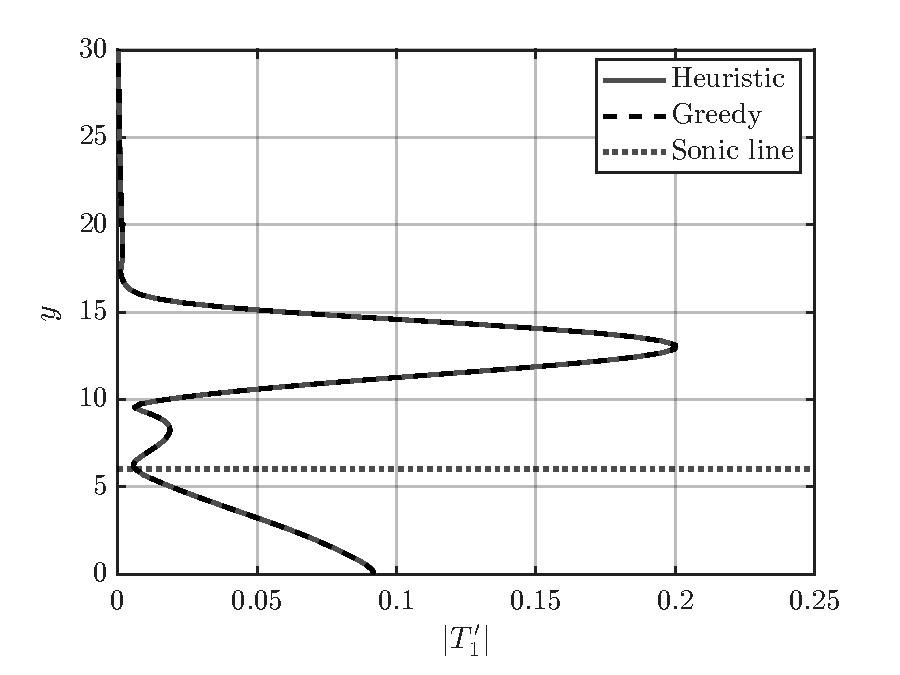
\includegraphics[width=1\linewidth]{figures/NOWNS_Zhu_T1_0500_bw.pdf}
        \caption{$T_1'$ at $Re_x=6.92\times10^5$}\label{fig:NOWNS-Zhu-T1-0500}
    \end{subfigure}
    \begin{subfigure}[b]{0.48\textwidth}
        \centering
        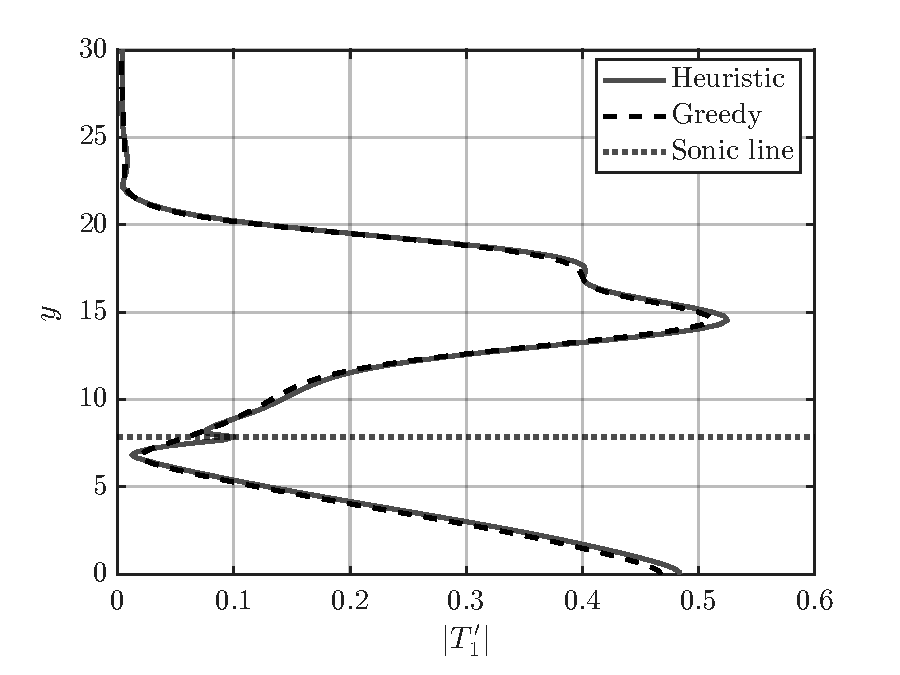
\includegraphics[width=1\linewidth]{figures/NOWNS_Zhu_T1_2501_bw.pdf}
        \caption{$T_1'$ at $Re_x=1.21\times10^6$}\label{fig:NOWNS-Zhu-T1-2501}
    \end{subfigure}\\
    \begin{subfigure}[b]{0.48\textwidth}
        \centering
        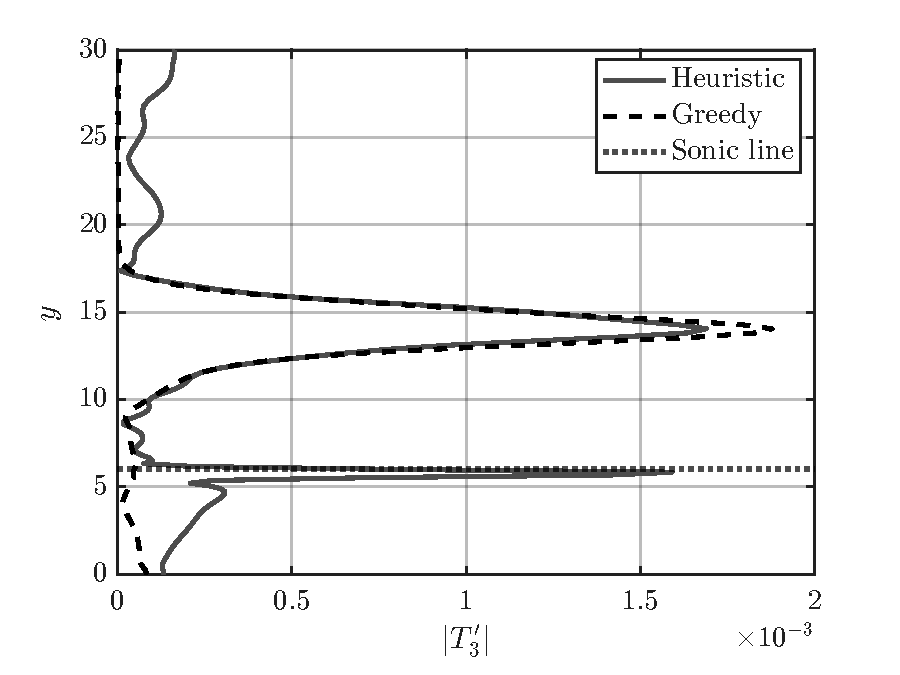
\includegraphics[width=1\linewidth]{figures/NOWNS_Zhu_T3_0500_bw.pdf}
        \caption{$T_3'$ at $Re_x=6.92\times10^5$}\label{fig:NOWNS-Zhu-T3-0500}
    \end{subfigure}
    \begin{subfigure}[b]{0.48\textwidth}
        \centering
        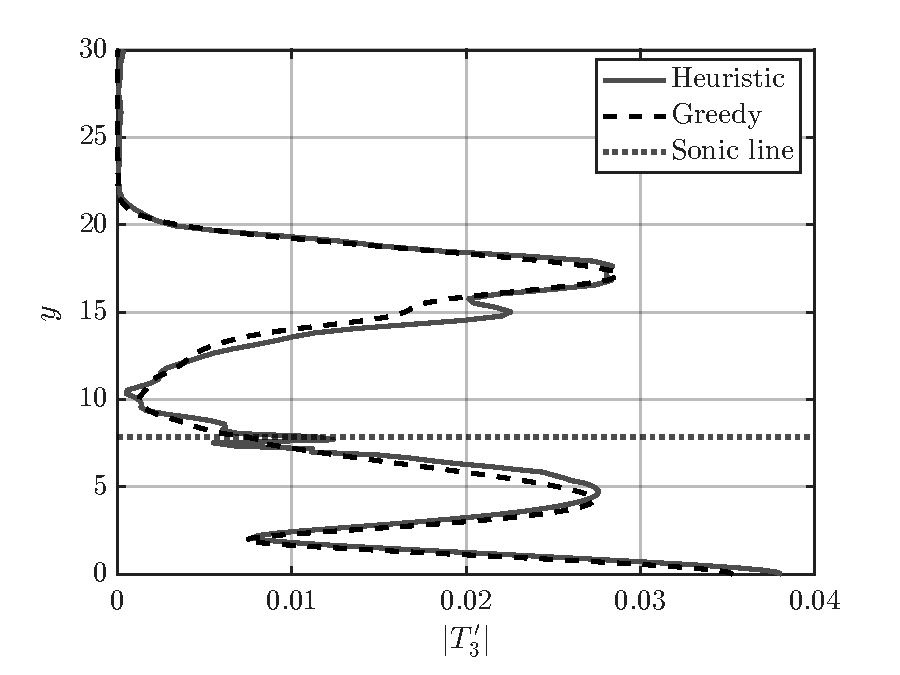
\includegraphics[width=1\linewidth]{figures/NOWNS_Zhu_T3_2501_bw.pdf}
        \caption{$T_3'$ at $Re_x=1.21\times10^6$}\label{fig:NOWNS-Zhu-T3-2501}
    \end{subfigure}    
    \caption{Temperature profiles for modes $T_1'$ and $T_3'$ computed for nonlinear evolution of Mack's second mode.}
    \label{fig:NOWNS-Zhu-01}
\end{figure}


% \begin{figure}
%     \centering
%     \begin{subfigure}[b]{0.48\textwidth}
%         \centering
%         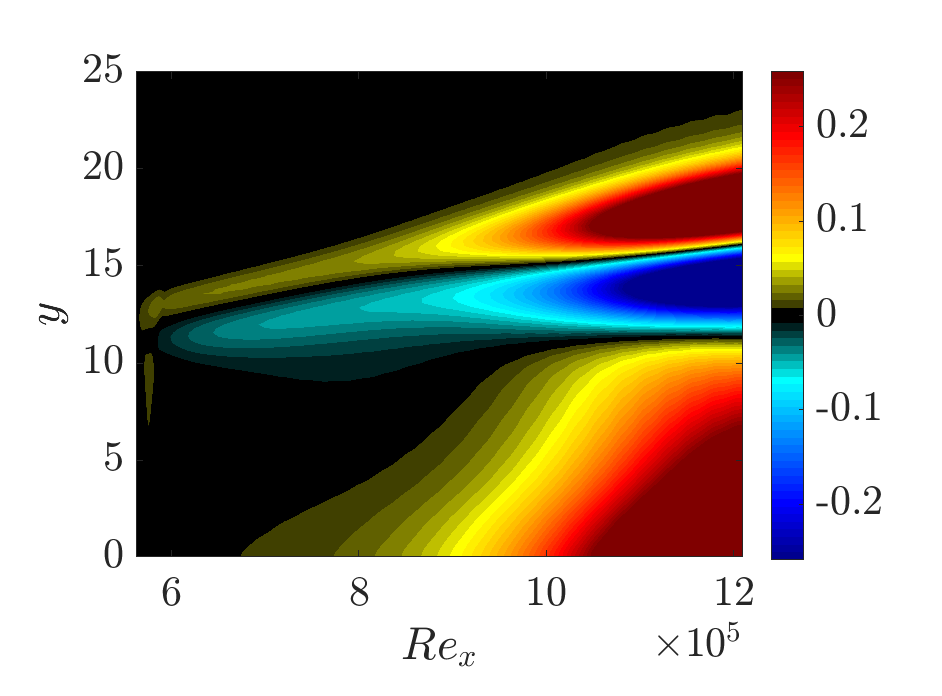
\includegraphics[width=1\linewidth]{figures/NOWNS_Zhu_Heuristic_T0.pdf}
%         \caption{Heuristic $T_0'$}\label{fig:NOWNS-Zhu-Heuristic-T0}
%     \end{subfigure}
%     \begin{subfigure}[b]{0.48\textwidth}
%         \centering
%         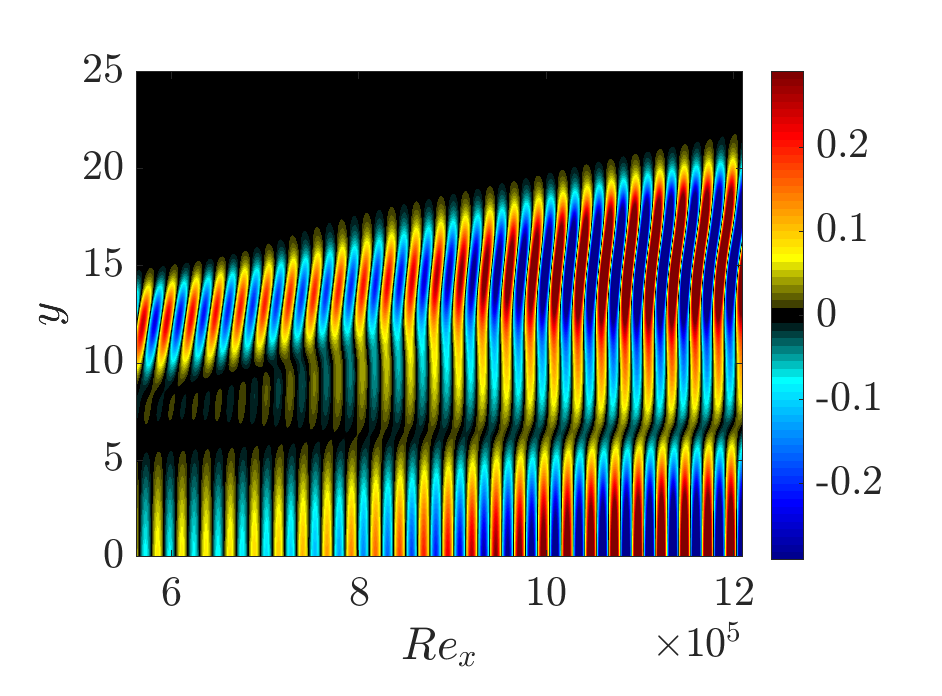
\includegraphics[width=1\linewidth]{figures/NOWNS_Zhu_Heuristic_T1.pdf}
%         \caption{Heuristic $T_1'$}\label{fig:NOWNS-Zhu-Heuristic-T1}
%     \end{subfigure}
%     \caption{Temperature contours for $T_0'$ and $T_1'$ for nonlinear evolution of Mack's second mode with heuristic recursion parameter selection.}
%     \label{fig:NOWNS-Zhu-01}
% \end{figure}

% \begin{figure}
%     \begin{subfigure}[b]{0.48\textwidth}
%         \centering
%         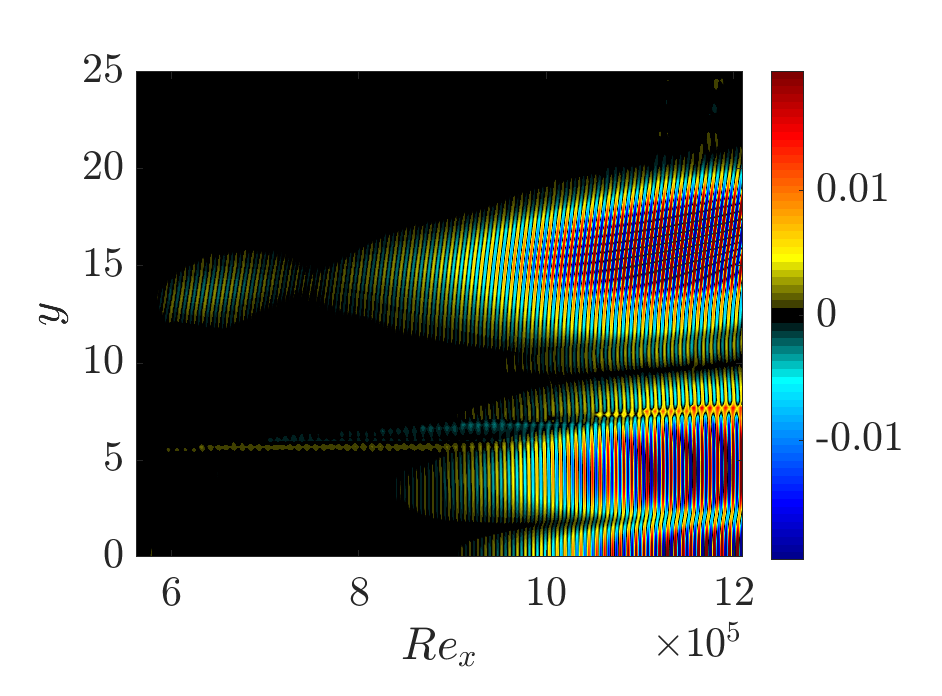
\includegraphics[width=1\linewidth]{figures/NOWNS_Zhu_Heuristic_T3.pdf}
%         \caption{Heuristic $T_3'$}\label{fig:NOWNS-Zhu-Heuristic-T3}
%     \end{subfigure}
%     \begin{subfigure}[b]{0.48\textwidth}
%         \centering
%         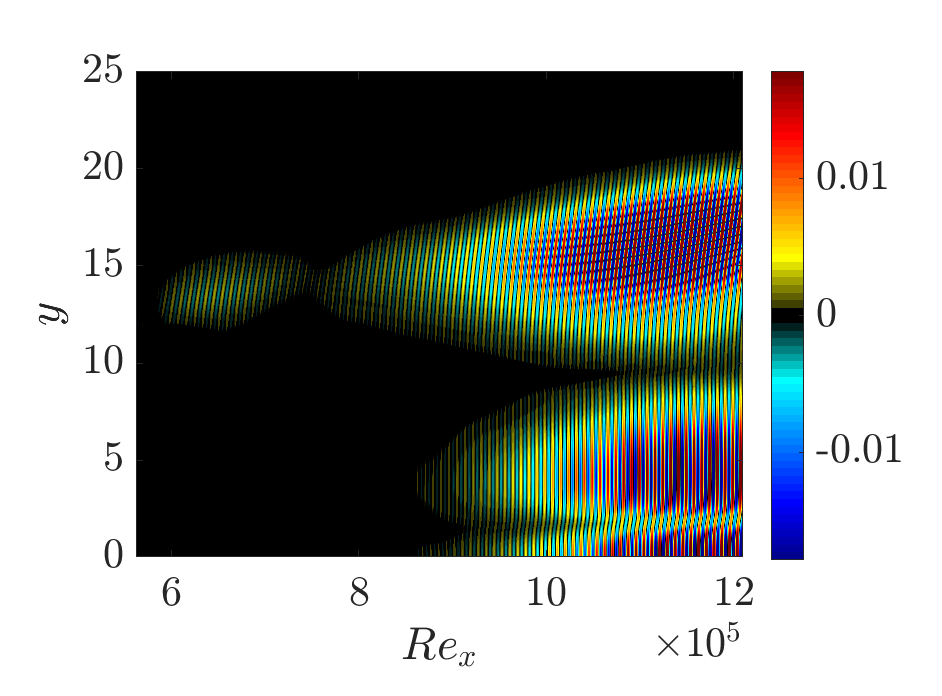
\includegraphics[width=1\linewidth]{figures/NOWNS_Zhu_Greedy_T3.pdf}
%         \caption{Greedy $T_3'$}\label{fig:NOWNS-Zhu-Greedy-T3}
%     \end{subfigure}\\
%     \caption{Temperature contours for $T_3'$ for nonlinear evolution of Mack's second mode with heuristic and greedy recursion parameter selection. Note that the non-physical grid effects disappear when using greedy selection.}
%     \label{fig:NOWNS-Zhu-3}
% \end{figure}

% \subsection{Linear calculations for 2D low-speed and high-speed boundary-layer flows}

% For our 2D low-speed boundary-layer flow we demonstration in figure~\ref{fig:Bertolotti-Power} that updating the recursion parameters at each step of the march yields a relatively constant value of the objective function in $x$. We consider two approaches: (i) compute all eigenvalues of $M$ only at the inlet and update these recursion parameters at each subsequent station, and (ii) compute all eigenvalues of $M$ and perform the greedy algorithm again at regular intervals, while updating the recursion parameters for subsequent stations based on the closest left station. We see that both approaches yields small values of the objective function, but that the second approach (which entails a higher computational cost) yields smaller values of the objective function. Figure~\ref{fig:Pruett-Power} demonstrates the interpolation procedure for the Mach 4.5 boundary-layer flow. The number of left- and right-going characteristics changes 23 times between $Re_x=6.4\times10^5$ and $Re_x=1.44\times10^6$, so that we must compute all the eigenvalues of $M$ 23 times, which increases the cost of the greedy approach relative to subsonic flows.

% \begin{figure}
%     \centering
%     \begin{subfigure}[b]{0.48\textwidth}
%         \centering
%         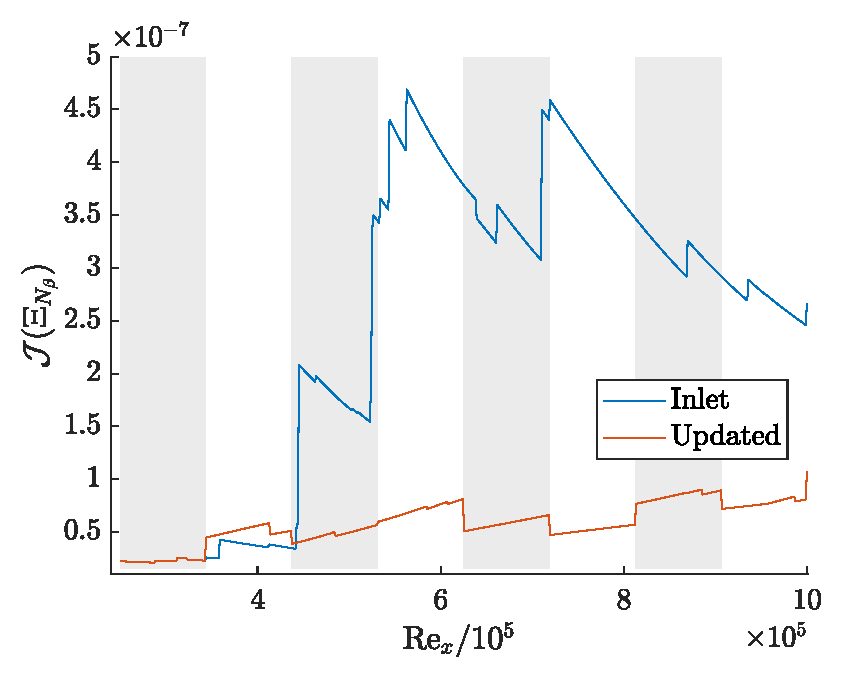
\includegraphics[width=1\linewidth]{figures/Bertolotti_Power_Update.pdf}
%         \caption{2D low-speed boundary-layer flow with $N_\beta=20$.}
%         \label{fig:Bertolotti-Power}
%     \end{subfigure}
%     \begin{subfigure}[b]{0.48\textwidth}
%         \centering
%         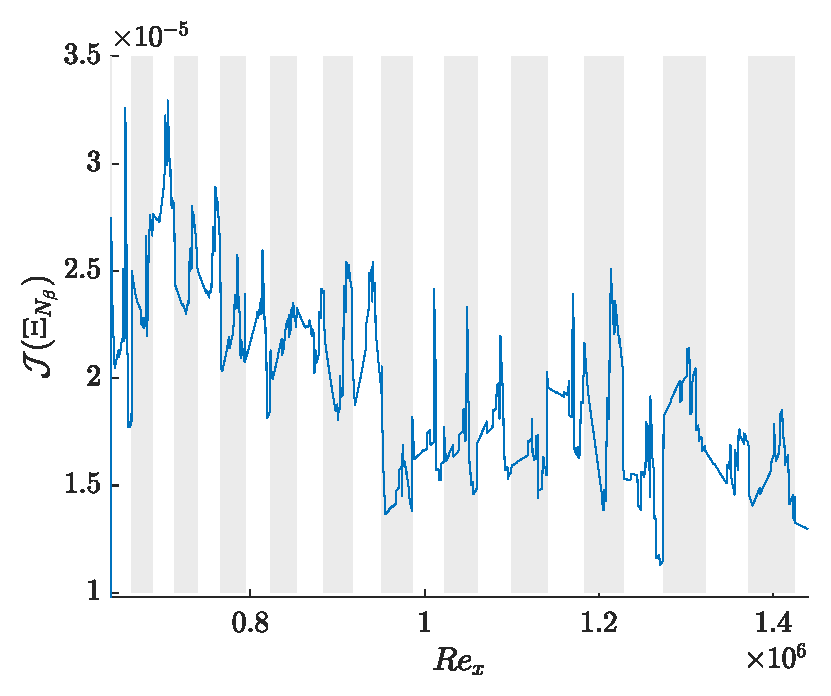
\includegraphics[width=1\linewidth]{figures/Pruett_Power_2.pdf}
%         \caption{2D high-speed boundary-layer flow with $N_\beta=15$.}
%         \label{fig:Pruett-Power}
%     \end{subfigure}
%     \caption{Objective function as a function of streamwise station using MATLAB \texttt{eigs} to update recursion parameters.}
% \end{figure}


\section{Conclusion}


Through numerical analyses and experiments, we have compared the convergence properties of the recursive filters used by OWNS-P and OWNS-R, and introduced a greedy algorithm to automatically choose recursion parameters that ensure rapid convergence of the filter error. Although we have used the OWNS label, which refers to the method when generalized to the linearized Navier-Stokes equations, we would like to emphasize that all of the analyses also apply to systems of linear first-order hyperbolic equation, and that the greedy algorithm could also be applied to such systems. In summary, we showed that OWNS-P has superior error convergence properties, so that there exist recursion parameter sets for which OWNS-P is fully converged, while OWNS-R is not. Conversely, if OWNS-R is fully converged, then OWNS-P must also be fully converged. We found for boundary-layer flows that the heuristic parameter selection that yields a stable and accurate OWNS-P march is inaccurate and unstable for OWNS-R. The underlying issue appears to be the rounding errors associated with finite precision arithmetic introduced when factoring the polynomial~\eqref{eq:owns-r-polynomial} and with solving the system~\eqref{eq:filter-r}. Therefore, future work should investigate how to modify the OWNS-R routine to minimize the impact of this rounding error, for example, using higher precision arithmetic.

We demonstrated for linear and nonlinear disturbance evolution in boundary-layer flows that our proposed greedy algorithm yields faster error convergence and a reduced computational cost relative to heuristic parameter selection. We further demonstrated the heuristic NOWNS for high-speed boundary-layer flows introduces spurious numerical oscillations, which are eliminated using the greedy algorithm, suggesting that the existing heuristic routine is not sufficiently accurate. We compared the greedy and heuristic recursion parameter sets, and highlighted that greedy OWNS converges more quickly since it places its eigenvalues more efficiently, and we note that future work could use greedy parameter selection to help tune the heuristic routines. We further emphasize that the heuristic parameter selection routine requires an analytical approximation to the eigenvalues of the governing equations (e.g., the eigenvalues of the Euler equations linearized about a uniform flow can be computed analytically) and a method to use this approximation to construct sets of convergence recursion parameters. For equations of interest, an analytical approximation to the eigenvalues may not exist, and even if it does, it may not be obvious how to use the expression to construct convergent recursion parameters sets. The greedy algorithm allows for automatic recursion parameter selection without the need for analytical approximations, which will allow the OWNS approach to be applied more easily to new systems of linear first-order hyperbolic equations. Finally, we note that this work focused only on flows with a single inhomogeneous direction (the wall-normal direction), and we note that the approach may not extend readily to flows with two or more inhomogeneous directions due to the increased grid size, and so future work should explore how to adapt the greedy algorithm for such cases.


\section*{Acknowledgments}

This work has been supported by The Boeing Company through the Strategic Research and Development Relationship
Agreement CT-BA-GTA-1.

\appendix
\section{Proofs}~\label{app:Proofs}

\begin{proof}[Proof of proposition~\ref{prop:errBoundTriangle}]
    $R_{N_\beta}$ comprises four blocks, where the diagonal blocks are square and the off-diagonal block are conformal with them for partitioning. Recall from~\eqref{eq:approxProjectRMat} that $R_{N_\beta}$ is defined as the inverse of another matrix, so that obtaining a simplified expression for $R_{N_\beta}^{-1}$ is straightforward, while it is more challenging for $R_{N_\beta}$. Define $S=R_{N_\beta}^{-1}$, so that it can be inverted blockwise as
    \[
        R_{N_\beta}=S^{-1}=
        \begin{bmatrix}
            S_{++} & S_{+-}\\
            S_{-+} & S_{--}
        \end{bmatrix}^{-1}
        =
        \begin{bmatrix}
            [S^{-1}]_{++} & [S^{-1}]_{+-}\\
            [S^{-1}]_{-+} & [S^{-1}]_{--}
        \end{bmatrix}.
    \]
    Then
    \[
    E-R_{N_\beta}E R_{N_\beta}^{-1}
    =
    E-S^{-1} E S
    =
    \begin{bmatrix}
            ([S^{-1}]_{++})(S_{++})- I_{++} &
            ([S^{-1}]_{++})(S_{+-})\\
            ([S^{-1}]_{-+})(S_{++}) &
            ([S^{-1}]_{-+})(S_{+-})
        \end{bmatrix}.
    \]
    and by the triangle inequality
    \begin{align}
    \begin{split}
    \|E-R_{N_\beta}^{-1}E R_{N_\beta}\|
    &\leq
    \|([S^{-1}]_{++})(S_{++}) - I_{++}\|
    +\|([S^{-1}]_{++})(S_{+-})\|\\
    &+\|([S^{-1}]_{-+})(S_{++})\|
    +\|([S^{-1}]_{-+})(S_{+-})\|.
    \end{split}
    \label{eq:errBoundTriangle}
    \end{align} 
    Next we have
    \begin{align*}
        [S^{-1}]_{++}
        &=(S_{++}-S_{+-}S_{--}^{-1}S_{-+})^{-1},\\
        &=(I_{++}-F_{++}V_{++}^{-1}V_{+-}F_{--}^{-2}V_{--}^{-1}V_{-+}F_{++})^{-1}\\
        [S^{-1}]_{-+}
        &=-S_{--}^{-1}S_{-+}[S^{-1}]_{++}\\
        &=-F_{--}^{-1}V_{--}^{-1}V_{-+}F_{++}(I_{++}-F_{++}V_{++}^{-1}V_{+-}F_{--}^{-2}V_{--}^{-1}V_{-+}F_{++})^{-1},
    \end{align*}
    while $S_{++}=I_{++}$ and $S_{-+}=F_{++}V_{++}^{-1}V_{+-}F_{--}^{-1}$ so that
    \begin{subequations}
    \begin{align}
    \begin{split}
        \|([S^{-1}]_{++})(S_{++})- I_{++}\|
        &\leq
        \|F_{++}V_{++}^{-1}V_{+-}F_{--}^{-1}\|\times
        \|F_{--}^{-1}V_{--}^{-1}V_{-+}F_{++}\|\\
        &\times
        \|(I_{++}-F_{++}V_{++}^{-1}V_{+-}F_{--}^{-2}V_{--}^{-1}V_{-+}F_{++})^{-1}\|
    \end{split}\\
    \begin{split}
        \|([S^{-1}]_{++})(S_{+-})\|
        &\leq
        \|F_{++}V_{++}^{-1}V_{+-}F_{--}^{-1}\|\\
        &\times
        \|(I_{++}-F_{++}V_{++}^{-1}V_{+-}F_{--}^{-2}V_{--}^{-1}V_{-+}F_{++})^{-1}\|,
    \end{split}\\
    \begin{split}
        \|([S^{-1}]_{-+})(S_{++})\|
        &\leq\|F_{--}^{-1}V_{--}^{-1}V_{-+}F_{++}\|\\
        &\times\|(I_{++}-F_{++}V_{++}^{-1}V_{+-}F_{--}^{-2}V_{--}^{-1}V_{-+}F_{++})^{-1}\|,
    \end{split}\\
    \begin{split}
        \|([S^{-1}]_{-+})(S_{+-})\|
        &\leq\|F_{--}^{-1}V_{--}^{-1}V_{-+}F_{++}\|
        \times\|F_{++}V_{++}^{-1}V_{+-}F_{--}^{-1}\|\\
        &\times\|(I_{++}-F_{++}V_{++}^{-1}V_{+-}F_{--}^{-2}V_{--}^{-1}V_{-+}F_{++})^{-1}\|.
    \end{split}
    \end{align}
    \label{eq:errBoundBlockInverse}
    \end{subequations}
    Substituting~\eqref{eq:errBoundBlockInverse} into~\eqref{eq:errBoundTriangle} yields~\eqref{eq:errBoundTriangleFinal}.
\end{proof}


\section{Special cases of singular $A$}\label{app:singular}

If $A$ is singular, then we obtain
\begin{equation}
    \tilde{A}=\begin{bmatrix}
        A_{++} & 0      & 0\\
        0      & A_{--} & 0\\
        0      & 0      & A_{00}
    \end{bmatrix}
\end{equation}
for diagonal $A_{++}\in\mathbb{R}^{N_+\times N_+}$ with $A_{++}>0$, $A_{--}\in\mathbb{R}^{N_-\times N_-}$ with $A_{--}<0$, and $A_{00}\in\mathbb{R}^{N_0\times N_0}$ with $A_{00}=0$, where $N_++N_-+N_0=N$. Then we define
\begin{subequations}
\begin{equation}
\tilde{A}_{\pm\pm}=\begin{bmatrix}
    A_{++} & 0     \\
    0      & A_{--}
\end{bmatrix}
\end{equation}
and
\begin{align}
\begin{split}
\tilde{L}(s)
&=\begin{bmatrix}
    L_{\pm\pm} & L_{\pm0}\\
    L_{0\pm}   & L_{00}
\end{bmatrix}\\
&=\begin{bmatrix}
    s I_{\pm\pm}+\sum_{j=2}^d i\omega_j\tilde{B}_{j,\pm\pm}+\tilde{C}_{\pm\pm} &
    \sum_{j=2}^d i\omega_j\tilde{B}_{j,\pm0}+\tilde{C}_{\pm0}\\
    \sum_{j=2}^d i\omega_j\tilde{B}_{j,0\pm}+\tilde{C}_{0\pm} &
    s I_{00} + \sum_{j=2}^d i\omega_j\tilde{B}_{j,00}+\tilde{C}_{00}
\end{bmatrix},
\end{split}
\end{align}
\end{subequations}
so that
\begin{subequations}
    \begin{align}
        \tilde{A}_{\pm\pm}\frac{d\hat{\bm{\phi}}_{\pm}}{d x}
        &=L_{\pm\pm}\hat{\bm{\phi}}_{\pm}+L_{\pm0}\hat{\bm{\phi}}_0+\hat{\bm{f}}_{\phi,\pm}\\
        0
        &=L_{0\pm}\hat{\bm{\phi}}_{\pm}+L_{00}\hat{\bm{\phi}}_0+\hat{\bm{f}}_{\phi,0}.
    \end{align}
\end{subequations}
The zero eigenvalues, $\tilde{A}_{00}$, correspond to points in the base flow where the streamwise velocity is exactly zero or sonic. In practice, unless a grid point is placed exactly on the sonic line, we will have $\tilde{A}_{00}$ associated with wall boundary-conditions only, so that $L_{00}$ will be invertible and we can eliminate $\hat{\bm{\phi}}_0$ as
\begin{equation}
    \hat{\bm{\phi}}_0=-L_{00}^{-1}(L_{0\pm}\hat{\bm{\phi}}_{\pm}+\hat{\bm{f}}_{\phi,0}).
\end{equation}
We then define
\begin{equation}
    M=\tilde{A}_{\pm\pm}^{-1}(L_{\pm\pm}-L_{\pm0}L_{00}^{-1}L_{0\pm}),\quad \hat{\bm{g}}=\tilde{A}_{\pm\pm}^{-1}(\hat{\bm{f}}_{\phi,\pm}-L_{\pm0}L_{00}^{-1}\hat{\bm{f}}_{\phi,0}),
    \end{equation}
to obtain the ODE
\begin{equation}
    \frac{d\hat{\bm{\phi}}}{d x}=M\hat{\bm{\phi}}_{\pm}+\hat{\bm{g}},
\end{equation}
which can be treated as in the non-singular case.
\section{Rounding errors in OWNS-R}~\label{app:Rounding}

In theory, the OWNS-R error decreases with increasing $N_\beta$ if both $\|F_{++}\|$ and $\|F_{--}^{-1}\|$ decrease. However, as discussed in Remark~\ref{rmk:rounding}, computing $\beta_j^*$ numerically (e.g., via \texttt{roots} in MATLAB) introduces rounding errors that prevent convergence. To estimate this rounding error for the 3D oblique-wave breakdown of low-speed Blasius boundary-layer flow in Section~\ref{sec:greedySingle}, we choose random complex numbers $c_k = a_k+ib_k$ with $a_k,b_k\in[-1,1]$ for $k=1,\dots,100$ and compute the relative error in the polynomial approximation as
\begin{equation}
    \max_{k=1,\dots,100}
    \frac{
    |2\prod_{j=1}^{N_\beta}(c_k-\beta_*^j)
    -\prod_{j=1}^{N_\beta}(c_k-\beta_-^j)
    -\prod_{j=1}^{N_\beta}(c_k-\beta_+^j)|}
    {|\prod_{j=1}^{N_\beta}(c_k-\beta_-^j)
    -\prod_{j=1}^{N_\beta}(c_k-\beta_+^j)|}.
\end{equation}
Figure~\ref{fig:poly_err} shows that this error is an increasing function of $N_\beta$, and future work should investigate how to minimize the impact of this rounding error on OWNS-R.
\begin{figure}
    \centering
    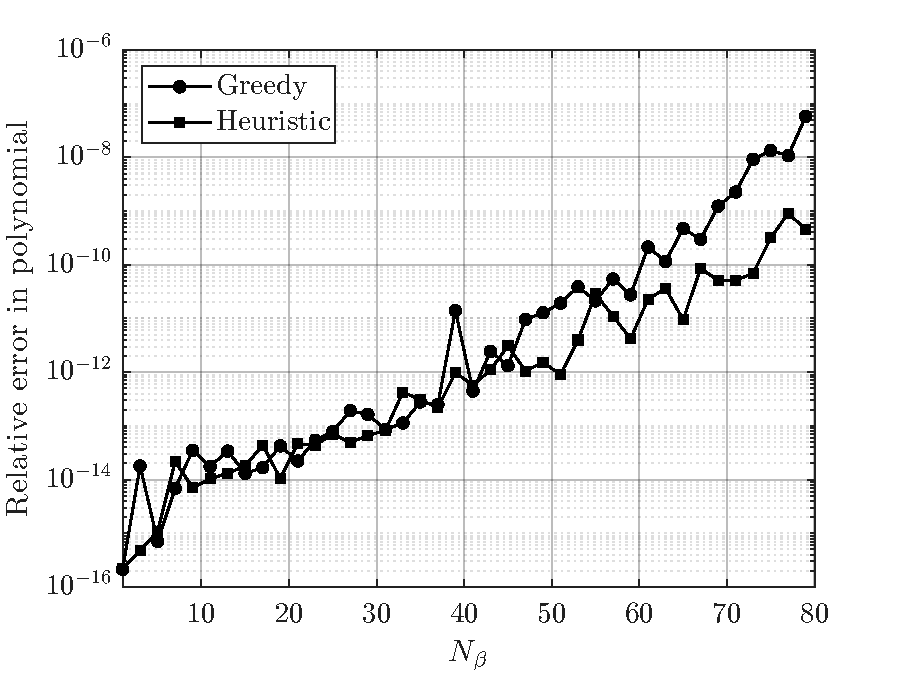
\includegraphics[width=0.5\linewidth]{figures/Oblique_Poly_Err_bw.pdf}
    \caption{The rounding error associated with computing $\beta_*^j$ for OWNS-R increases with increasing $N_\beta$. Demonstration for 3D oblique-wave breakdown of low-speed Blasius boundary-layer flow.}
    \label{fig:poly_err}
\end{figure}

\bibliographystyle{siamplain}
\bibliography{ownslibrary}
\end{document}
